

\documentclass[a4paper,fleqn]{cas-dc}


\usepackage[numbers,sort&compress]{natbib}

\usepackage{booktabs}
\usepackage{multirow}
\usepackage{makecell}
\usepackage{amsmath}
\usepackage{amssymb}
\usepackage{array}
\usepackage{xcolor}
\usepackage{lineno}
\usepackage{placeins}   % provides \FloatBarrier
\usepackage{float}      % provides [H] specifier
\usepackage{capt-of}    % provides \captionof for non-floating captions
\usepackage{xurl}       % allows long URLs to break across lines
\usepackage{tikz}
\usetikzlibrary{shapes.geometric, arrows.meta, positioning, calc, backgrounds}

\graphicspath{{figs/}}

\hyphenation{video-fluoro-scopy video-fluoro-scopic semi-super-vised}


\definecolor{lowlabel}{RGB}{225, 245, 238}
\definecolor{highlabel}{RGB}{250, 236, 231}
\definecolor{sslpurple}{RGB}{238, 237, 254}
\definecolor{graybox}{RGB}{241, 239, 232}
\definecolor{accentgreen}{RGB}{29, 158, 117}
\definecolor{accentorange}{RGB}{216, 90, 48}
\definecolor{pool1}{RGB}{232, 225, 247}
\definecolor{pool2}{RGB}{210, 196, 240}
\definecolor{pool3}{RGB}{182, 160, 228}

\newcommand{\makefigone}{%
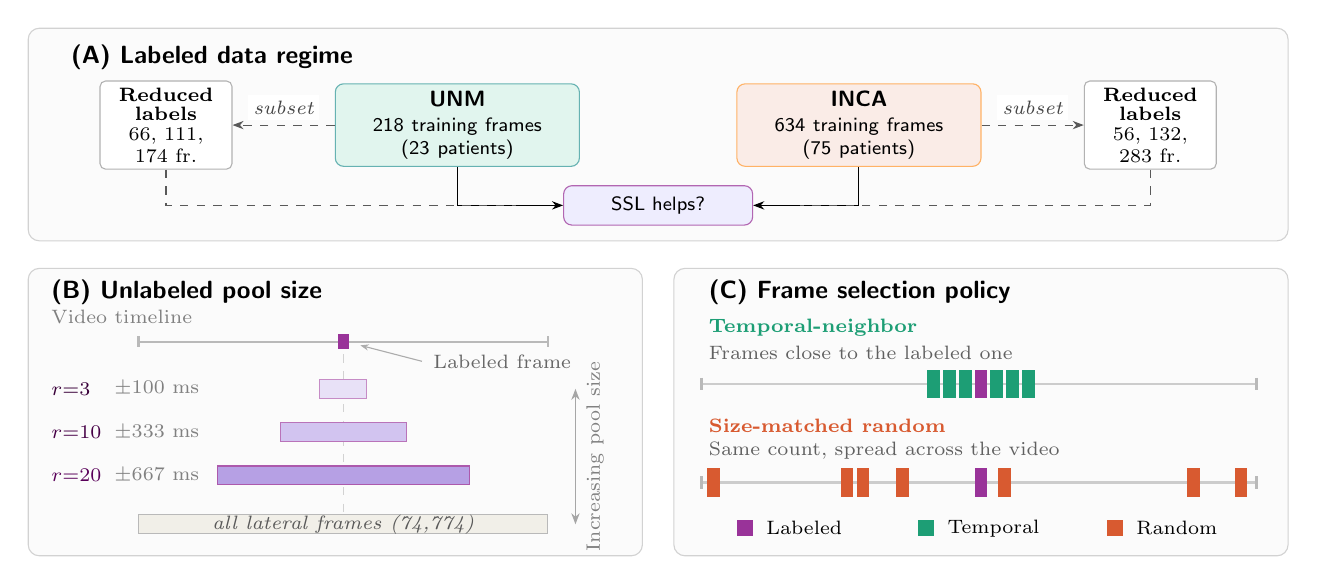
\begin{tikzpicture}[
  x=1cm,
  y=1cm,
  font=\sffamily\footnotesize,
  every node/.style={inner sep=2.5pt},
  panel/.style={draw=gray!35, rounded corners=4pt, fill=gray!3},
  box/.style={draw, rounded corners=3pt, minimum width=3.1cm, minimum height=0.85cm, text width=2.8cm, align=center},
  sslbox/.style={draw, rounded corners=3pt, fill=sslpurple, draw=violet!60, minimum width=2.4cm, minimum height=0.50cm, align=center},
  >={Stealth[length=4pt]}
]


\draw[panel] (-8.0, 0.15) rectangle (8.0, -2.55);
\draw[panel] (-8.0, -2.90) rectangle (-0.2, -6.55);
\draw[panel] ( 0.2, -2.90) rectangle ( 8.0, -6.55);

\node[font=\sffamily\small\bfseries, anchor=west] at (-7.55, -0.22) {(A) Labeled data regime};

\node[draw=gray!60, rounded corners=2pt, fill=white, align=center,
      font=\scriptsize, text width=1.5cm, minimum height=0.85cm] (unmsub)
      at (-6.25, -1.08) {%
  \textbf{Reduced}\\[-1pt]
  \textbf{labels}\\[-1pt]
  66, 111, 174 fr.
};

\node[box, fill=lowlabel, draw=teal!60] (unm) at (-2.55, -1.08) {%
  \textbf{UNM}\\[1pt]
  \scriptsize 218 training frames\\[-1pt]
  \scriptsize (23 patients)
};

\node[box, fill=highlabel, draw=orange!60] (inca) at (2.55, -1.08) {%
  \textbf{INCA}\\[1pt]
  \scriptsize 634 training frames\\[-1pt]
  \scriptsize (75 patients)
};

\node[draw=gray!60, rounded corners=2pt, fill=white, align=center,
      font=\scriptsize, text width=1.5cm, minimum height=0.85cm] (incasub)
      at (6.25, -1.08) {%
  \textbf{Reduced}\\[-1pt]
  \textbf{labels}\\[-1pt]
  56, 132, 283 fr.
};

\draw[->, dashed, thin, gray!70!black] (unm.west) -- (unmsub.east);
\draw[->, dashed, thin, gray!70!black] (inca.east) -- (incasub.west);

\node[fill=white, inner sep=2pt,
      font=\scriptsize\itshape, text=gray!55!black]
      (tagunm) at ($(unm.west)!0.5!(unmsub.east) + (0,0.22)$) {subset};
\node[fill=white, inner sep=2pt,
      font=\scriptsize\itshape, text=gray!55!black]
      (taginca) at ($(inca.east)!0.5!(incasub.west) + (0,0.22)$) {subset};

\node[sslbox] (sslq) at (0, -2.10) {\scriptsize SSL helps?};

\coordinate (joinL) at (-1.80, -2.10);
\coordinate (joinR) at ( 1.80, -2.10);

\draw[thin] (unm.south)  |- (joinL);
\draw[thin] (inca.south) |- (joinR);

\draw[dashed, thin, gray!70!black] (unmsub.south)  |- (joinL);
\draw[dashed, thin, gray!70!black] (incasub.south) |- (joinR);

\draw[->, thin] (joinL) -- (sslq.west);
\draw[->, thin] (joinR) -- (sslq.east);

\node[font=\sffamily\small\bfseries, anchor=west] at (-7.80, -3.20)
      {(B) Unlabeled pool size};

\draw[dashed, gray!35, very thin] (-4.00, -3.78) -- (-4.00, -6.23);

\draw[thick, gray!55] (-6.60, -3.83) -- (-1.40, -3.83);
\draw[thick, gray!55] (-6.60, -3.76) -- (-6.60, -3.90);
\draw[thick, gray!55] (-1.40, -3.76) -- (-1.40, -3.90);
\node[font=\scriptsize, gray, anchor=west] at (-7.80, -3.52)
      {Video timeline};

\fill[violet!80] (-4.07, -3.93) rectangle (-3.93, -3.73);
\draw[-{Stealth[length=3pt]}, gray!65, thin, shorten >=2pt]
  (-3.00, -4.08) -- (-3.85, -3.86);
\node[font=\scriptsize, gray!80!black, anchor=west] at (-2.95, -4.08)
      {Labeled frame};

\node[font=\scriptsize\bfseries, violet!45!black, anchor=west] at (-7.80, -4.43)
      {$r{=}3$};
\node[font=\scriptsize, gray, anchor=west] at (-7.00, -4.43) {$\pm 100$ ms};
\fill[pool1, draw=violet!45, thin] (-4.30, -4.55) rectangle (-3.70, -4.31);

\node[font=\scriptsize\bfseries, violet!55!black, anchor=west] at (-7.80, -4.98)
      {$r{=}10$};
\node[font=\scriptsize, gray, anchor=west] at (-7.00, -4.98) {$\pm 333$ ms};
\fill[pool2, draw=violet!55, thin] (-4.80, -5.10) rectangle (-3.20, -4.86);

\node[font=\scriptsize\bfseries, violet!70!black, anchor=west] at (-7.80, -5.53)
      {$r{=}20$};
\node[font=\scriptsize, gray, anchor=west] at (-7.00, -5.53) {$\pm 667$ ms};
\fill[pool3, draw=violet!65, thin] (-5.60, -5.65) rectangle (-2.40, -5.41);

\fill[graybox, draw=gray!55, thin] (-6.60, -6.27) rectangle (-1.40, -6.03);
\node[font=\scriptsize\itshape, gray!70!black] at (-4.00, -6.15)
      {all lateral frames (74{,}774)};

\draw[<->, gray!70, thin] (-1.05, -4.43) -- (-1.05, -6.15);
\node[font=\scriptsize, gray, rotate=90, align=center] at (-0.80, -5.29)
      {Increasing pool size};


\node[font=\sffamily\small\bfseries, anchor=west] at (0.55, -3.20)
      {(C) Frame selection policy};

\node[font=\scriptsize\bfseries, accentgreen, anchor=west] at (0.55, -3.65)
      {Temporal-neighbor};
\node[font=\scriptsize, gray!75!black, anchor=west] at (0.55, -3.97)
      {Frames close to the labeled one};
\draw[thick, gray!40] (0.55, -4.37) -- (7.60, -4.37);
\draw[thick, gray!55] (0.55, -4.29) -- (0.55, -4.45);
\draw[thick, gray!55] (7.60, -4.29) -- (7.60, -4.45);
\fill[violet!80] (4.02, -4.55) rectangle (4.18, -4.19);
\foreach \x in {3.5, 3.70, 3.90, 4.50, 4.3, 4.5, 4.7} {
  \fill[accentgreen] (\x-0.08, -4.55) rectangle (\x+0.08, -4.19);
}

\node[font=\scriptsize\bfseries, accentorange, anchor=west] at (0.55, -4.90)
      {Size-matched random};
\node[font=\scriptsize, gray!75!black, anchor=west] at (0.55, -5.22)
      {Same count, spread across the video};
\draw[thick, gray!40] (0.55, -5.62) -- (7.60, -5.62);
\draw[thick, gray!55] (0.55, -5.54) -- (0.55, -5.70);
\draw[thick, gray!55] (7.60, -5.54) -- (7.60, -5.70);
\fill[violet!80] (4.02, -5.80) rectangle (4.18, -5.44);
\foreach \x in {0.70, 2.40, 2.60, 3.10, 4.40, 6.80, 7.40} {
  \fill[accentorange] (\x-0.08, -5.80) rectangle (\x+0.08, -5.44);
}

\fill[violet!80]    (1.00, -6.30) rectangle (1.20, -6.10);
\node[font=\scriptsize, anchor=west] at (1.28, -6.20) {Labeled};
\fill[accentgreen]  (3.30, -6.30) rectangle (3.50, -6.10);
\node[font=\scriptsize, anchor=west] at (3.58, -6.20) {Temporal};
\fill[accentorange] (5.70, -6.30) rectangle (5.90, -6.10);
\node[font=\scriptsize, anchor=west] at (5.98, -6.20) {Random};

\end{tikzpicture}%

}

\begin{document}
\let\WriteBookmarks\relax
\renewcommand{\topfraction}{0.85}
\renewcommand{\bottomfraction}{0.70}
\renewcommand{\textfraction}{0.10}
\renewcommand{\floatpagefraction}{0.60}

\shorttitle{SSL for Vertebra Segmentation in VFSS}

\shortauthors{S. Quispe Arias et~al.}

\title[mode=title]{Semi-supervised learning for cervical vertebra segmentation in videofluoroscopic swallowing studies}

\author[1]{Sebastian Quispe Arias}[orcid=0009-0009-1023-5851]
\ead{sarias@inf.puc-rio.br}
\credit{Methodology, Software, Formal analysis, Investigation, Visualization, Writing -- original draft}

\author[2]{Vin\'{i}cius Oliveira da Costa}
\ead{viniciuscosta@tecgraf.puc-rio.br}
\credit{Data curation}

\author[2]{Luiz Fernando Santos}
\ead{lsantos@tecgraf.puc-rio.br}
\credit{Methodology, Software, Supervision, Writing -- review \& editing}

\author[3]{Rayane Beltr\~{a}o Alves Cerqueira}
\ead{rayane.cerqueira@ensino.inca.gov.br}
\credit{Validation}

\author[3]{Andressa Silva de Freitas}
\ead{andressa.freitas@inca.gov.br}
\credit{Resources, Project administration, Writing -- review \& editing}

\author[2]{Yiselis Rodr\'{i}guez Vignon}
\cormark[1]
\ead{yiselisr@tecgraf.puc-rio.br}
\credit{Methodology, Supervision, Writing -- review \& editing}

\author[1,2]{Paulo Ivson}
\ead{psantos@tecgraf.puc-rio.br}
\credit{Conceptualization, Funding acquisition, Project administration, Supervision, Writing -- review \& editing}

\affiliation[1]{organization={Computer Science Department, Pontifical Catholic University of Rio de Janeiro (PUC-Rio)},
            addressline={Marqu\^{e}s de S\~{a}o Vicente Street, 225, G\'{a}vea},
            city={Rio de Janeiro},
            postcode={22451-900},
            state={RJ},
            country={Brazil}}

\affiliation[2]{organization={Tecgraf Institute of Technical-Scientific Software Development of PUC-Rio (Tecgraf/PUC-Rio), Pontifical Catholic University of Rio de Janeiro (PUC-Rio)},
            addressline={Marqu\^{e}s de S\~{a}o Vicente Street, 225, G\'{a}vea},
            city={Rio de Janeiro},
            postcode={22451-900},
            state={RJ},
            country={Brazil}}

\affiliation[3]{organization={National Cancer Institute (INCA)},
            city={Rio de Janeiro},
            country={Brazil}}

\cortext[1]{Corresponding author}

\begin{abstract}
\textbf{Background and Objective:} In videofluoroscopic swallowing studies (VFSS), cervical vertebrae serve as anatomical references for objective measurement of swallowing kinematics, but pixel-level annotation is costly and rarely available at scale.
Semi-supervised learning (SSL) can exploit unlabeled frames naturally present in VFSS video, but its role in this segmentation task remains underexplored.

\textbf{Methods:} This work systematically evaluates SSL for cervical vertebra segmentation using pseudo-labeling and Mean Teacher on two institutional datasets: the University of New Mexico (UNM) TalkBank subset with 218 training frames, and the Instituto Nacional de C\^ancer (INCA) subset with 634 training frames, totaling 342 training runs. The experiments varied the labeled-data budget, the size of the unlabeled pool, and the frame-selection strategy.

\textbf{Results:} Across all tested label budgets in both datasets, SSL achieved F1 comparable to or above supervised training, with Mean Teacher preserving segmentation quality under aggressive label reduction (F1 within 4.1 percentage points of the best supervised label-fraction result in INCA with 10\% labels, and within 1.3 points in UNM with 25\% labels).
The largest SSL gains occurred where the supervised baseline had not yet saturated: in UNM, Mean Teacher reached F1~=~0.860 vs supervised F1~=~0.801 ($\Delta$~=~+0.059 vs full-label baseline; +0.031 vs best supervised label-fraction result).
In INCA, SSL produced no improvement at 25\% labels and above; with only 10\% labels, Mean Teacher reached F1~=~0.865 over F1~=~0.844 ($\Delta$~=~+0.021).

\textbf{Conclusions:} These results indicate that SSL can be practically useful in low-label VFSS settings by exploiting unlabeled frames already present.
Beyond cervical vertebra segmentation, this work provides a basis for future applications of classical SSL to other VFSS segmentation targets and fluoroscopic imaging tasks where labeled data are scarce.
\end{abstract}

\begin{keywords}
Videofluoroscopy \sep cervical vertebra segmentation \sep semi-supervised learning \sep pseudo-labeling \sep Mean Teacher \sep label efficiency \sep unlabeled pool construction
\end{keywords}

\maketitle

\section{Introduction}
\label{sec:intro}

Videofluoroscopic swallowing studies (VFSS) are the most commonly used instrumental examination for evaluating dysphagia~\citep{ref_logemann}.
During a VFSS, continuous lateral X-ray images are recorded while the patient swallows.
Quantitative analysis of these recordings requires a stable anatomical frame of reference because head motion during swallowing displaces the imaged anatomy from frame to frame.
Cervical vertebrae fulfill this role across multiple downstream tasks: normalizing kinematic measurements across patients via the C2--C4 anatomical scalar~\citep{ref_molfenter,ref_steele_norms}, defining coordinate systems for hyoid bone tracking~\citep{ref_kim2021}, and serving as the reference point for region-of-interest definition for airway-invasion detection~\citep{ref_lee2020}.
For several of these tasks the full spatial extent of the vertebral region is needed, not only its corner landmarks: dynamic ROIs that follow head motion use the segmented spine as a reference~\citep{ref_lee2020}, and centroid-based measurement of hyoid displacement relative to the cervical spine requires a continuous mask~\citep{ref_kim2021}.
Automating vertebra segmentation would therefore support these downstream analyses simultaneously, but manual annotation of vertebral masks is costly and rarely available at scale.

This scarcity contrasts with the abundance of unlabeled frames: a single study generates hundreds to thousands of frames per patient.
Four recent reviews of VFSS analysis~\citep{ref_girardi2023,ref_shu_review,ref_sanjeevi2025,ref_fakhry2025} identify the scarcity of annotated data as a central challenge; most reported deep learning approaches are fully supervised.
This data regime naturally motivates semi-supervised learning (SSL), where a model is trained on both a small labeled set and a larger pool of unlabeled frames from the same videos.

The few existing deep learning approaches for cervical vertebra analysis in VFSS rely on supervised landmark regression, requiring thousands of annotated frames~\citep{ref_zhang2021,ref_li2024}.
More broadly, recent VFSS segmentation work has explored alternative paradigms for reducing annotation burden: \citet{ref_cubero2025} use an iterative labeling framework inspired by active learning, incorporating expert corrections of model predictions, whereas \citet{ref_zeng_ttt} use test-time prompt-guided training with MedSAM~\citep{ref_medsam}.
To the best of our knowledge, no prior work has applied the classical SSL setting (joint training on labeled and unlabeled data) to any segmentation task in VFSS.

Applying SSL to a new domain such as VFSS raises three practical questions that have not been addressed jointly in prior work.
First, the benefit of SSL is known to depend on the amount of available annotation, but the regime in which SSL meaningfully helps for vertebra segmentation in VFSS has not been characterized.
Second, general SSL research has shown that not all unlabeled examples contribute equally~\citep{ref_ren2020} and that performance can degrade with out-of-distribution unlabeled data~\citep{ref_oliver2018}; the appropriate size of an unlabeled pool constructed from VFSS video is therefore an open question.
Third, because VFSS frames are drawn from continuous video, frames close to the labeled ones in time are visually similar to them, while distant frames may depict different anatomical configurations during the swallowing sequence; whether temporal proximity should guide frame selection, or whether a size-matched random sample suffices, has not been systematically studied.
Although related dimensions have been examined in laparoscopic image segmentation~\citep{ref_fu2019} and in general-domain semi-supervised classification~\citep{ref_rdss2024}, their role in classical SSL for VFSS segmentation remains unexplored.

The contributions of this work are fourfold. First, this study presents a systematic evaluation of semi-supervised learning for cervical vertebra segmentation in VFSS, using pseudo-labeling and Mean Teacher across two institutions and multiple label budgets. At matched budgets, SSL achieved F1 comparable to or above supervised training, with measurable gains where supervised performance had not yet saturated. Second, the study characterizes SSL behavior along three design dimensions common to such pipelines: the labeled data regime, the unlabeled pool size, and the frame selection policy. Third, the SSL results are contextualized against six supervised architectures: five general-purpose models and a Kim-inspired BiFPN-U-Net(T) adapted from the VFSS literature; nnU-Net is additionally included as a self-configuring reference. Finally, this work introduces pixel-level vertebral masks for the UNM dataset, which will be publicly released for reproducibility and future research on cervical vertebra segmentation in VFSS.

\section{Related work}
\label{sec:related}

\subsection{Cervical vertebra analysis in VFSS}

Cervical vertebra segmentation has been studied in static lateral radiographs, where \citet{ref_alarif2018} proposed a fully automatic framework combining spinal-region localization, vertebra-center regression, and shape-aware segmentation of C3--C7 (Dice~=~0.84, shape error~=~1.69~mm), and in dynamic X-ray, where \citet{ref_santbrink2025} compared 2D and 2D+t models for C0--C7 segmentation and found that seven consecutive frames performed best among the evaluated 2D+t configurations.
Within VFSS, automated analysis of cervical vertebrae has been approached mainly through landmark localization and semantic segmentation.
\citet{ref_zhang2021} trained a two-stage CNN to localize C2--C4 corner landmarks, reporting a mean localization distance of 4.20~px on 70~healthy subjects.
\citet{ref_li2024} used a Full-HRNet for simultaneous detection of the hyoid bone and C2--C4 corners, reaching 2.38~px mean error.
Both output point coordinates rather than masks.
\citet{ref_cubero2025} localized ten regions of interest via an iterative nnU-Net with expert-in-the-loop corrections, reporting a mean error of 1.6~px on an independent test cohort of healthy participants.

On the segmentation side, \citet{ref_fujinaka} segmented cervical intervertebral disks with a patch-based CNN (F-measure~=~0.593).
\citet{ref_lee2020} segmented the cervical spinal column as a preprocessing step for airway-invasion detection.
\citet{ref_kim2021} used a BiFPN-U-Net(T) to segment hyoid, spine, and a reference coin for hyoid tracking (Dice~=~90.9\% across three classes).

In these works the spine is an auxiliary structure rather than the segmentation target.
In concurrent work, two foundation-model approaches address vertebrae directly: \citet{ref_zeng_ttt} apply test-time training on MedSAM to segment individual C1--C7 vertebrae among 12~anatomies (average Dice~=~0.868), with full annotations on a source domain and manual point prompts at test time; \citet{ref_zeng_distill2025} distill knowledge from multiple vision foundation models (MedSAM, RAD-DINO, MedCLIP) into a lightweight student for the same 12~anatomies, but training itself uses ground-truth masks.
None of these works uses the classical SSL setting of joint training on labeled and unlabeled data, and none studies unlabeled pool composition.

\subsection{Alternatives to full supervision in VFSS}

Several recent VFSS studies have explored alternatives to full supervision.
\citet{ref_bandini2022} demonstrated weakly-supervised bolus localization in VFSS using class activation maps, reducing annotation requirements for bolus detection, though their approach does not incorporate unlabeled data during training.
\citet{ref_martinovic2025} used self-supervised pre-training (contrastive random walk) to learn representations from unlabeled VFSS frames, but their downstream bolus segmentation is fully supervised, as unlabeled data are used only in the pretext task, not during segmentation training.
An unsupervised convolutional autoencoder for bolus and residue segmentation~\citep{ref_unsup_bolus2025} operates without any pixel-level annotations, achieving IoU of 61\% for bolus, but this lies at the opposite end of the supervision spectrum from SSL.
None of them jointly trains on labeled and unlabeled frames for segmentation.


\subsection{Semi-supervised medical image segmentation}

Teacher--student frameworks~\citep{ref_mean_teacher}, pseudo-labeling~\citep{ref_fixmatch}, and cross-pseudo supervision~\citep{ref_cps} have been applied to medical image segmentation in various organs~\citep{ref_ssl_survey,ref_han2024}, but not to VFSS. Recent extensions include multi-teacher consistency learning~\citep{ref_qiu2025} and uncertainty-aware collaborative learning based on pseudo-labels~\citep{ref_wang2026}.
\citet{ref_ren2020} showed that not all unlabeled examples contribute equally to SSL performance.
\citet{ref_oliver2018} demonstrated that SSL performance can degrade when unlabeled data are out-of-distribution.
More recent work on data selection~\citep{ref_rdss2024} further shows that the choice of which data to include affects SSL outcomes.
However, the data-selection studies cited above focus primarily on image classification with i.i.d.\ data; unlabeled pool composition for segmentation in medical video, where frames have an inherent temporal structure, remains underexplored.

In related fluoroscopic domains, \citet{ref_luo_smart2026} recently proposed SMART, a SAM3-based teacher--student framework with motion-aware consistency and progressive confidence regularization for coronary vessel segmentation in X-ray angiography video, achieving over 6 percentage points of Dice improvement with only 16 labeled videos.
Their work shows that teacher--student SSL can be effective in X-ray angiography video, but it does not study unlabeled pool composition or VFSS segmentation.
\citet{ref_fu2019} investigated the trade-off between labeled and unlabeled data quantity for Mean Teacher in laparoscopic liver segmentation, finding that more unlabeled data does not always improve performance.
However, they varied only the \emph{quantity} of unlabeled frames using random selection and did not compare different selection strategies or study the effect of temporal proximity.
The present work extends this line of inquiry by systematically varying both pool size and selection policy in a medical video domain with inherent temporal structure.

\section{Materials and methods}
\label{sec:method}

This study evaluates SSL on two datasets with distinct labeled-data regimes, varying the unlabeled pool size and comparing two frame selection policies, as shown in Fig.~\ref{fig:design}.

\begin{figure*}[!htbp]
  \centering
  \makefigone
  \caption{Experimental design. (A)~UNM and INCA datasets with distinct labeled-data regimes. (B)~Unlabeled pools constructed at six temporal radiuses plus an all-lateral pool. (C)~Frame-selection policies compared: temporal-neighbor and size-matched random.}
  \label{fig:design}
\end{figure*}

\FloatBarrier

\subsection{Datasets}

This work uses two VFSS datasets from different institutions.
The datasets differ in annotation volume, video length, and patient population. The contrast in annotation volume enables evaluation of SSL across distinct labeling regimes.
A summary is given in Table~\ref{tab:datasets}.

\subsubsection{UNM dataset}

The first dataset is a subset of the University of New Mexico (UNM) TalkBank Dysphagia database~\citep{ref_talkbank}, an open-access repository of clinically-acquired videofluoroscopic swallowing studies.
For this study, only adult patients were retained, yielding 35 lateral VFSS videos from 35 patients (one video per patient), with ages ranging from 21 to 97 years.
The patients span a range of medical conditions referred for dysphagia evaluation; this clinical heterogeneity introduces anatomical and physiological variability that is not explicitly controlled.
Each video contains one or more swallows.
The original UNM TalkBank videos switch from lateral to anteroposterior view near the end; this final segment was removed, since prior work on VFSS segmentation operates in the lateral view.
Ten frames per video were sampled for annotation. Frames in which the cervical vertebrae were not visible (due to motion blur, low contrast, or projection changes) were excluded without replacement, yielding 325 annotated frames from 350 candidates across 35 videos (8 videos retained fewer than 10 frames).
Binary masks of the C2--C4 cervical vertebral region were manually annotated in ImageJ by one of the authors, a graduate student without formal clinical training, using the freehand selection tool. The same author also participated in annotating the INCA dataset described next. Vertebrae were included when judged visible by the annotator.
While the underlying videos are publicly available, the vertebral masks are a contribution of the present study.

The 325 lateral frames were split by patient into 23~training, 5~validation, and 7~test videos, yielding 218~labeled training frames, 44 validation frames, and 63 test frames.

To assess annotation reliability, a clinical specialist (speech-language pathologist) from a collaborating institution independently segmented 20 selected UNM frames without access to the original masks.
Inter-annotator agreement, measured by the Dice coefficient between the two sets of annotations, was 0.854~$\pm$~0.062.

\subsubsection{INCA dataset}

The second dataset was collected at the Instituto Nacional de C\^ancer (INCA, Rio de Janeiro, Brazil) and was provided under an institutional data-sharing agreement that authorized its use for research purposes.
It consists of 234 lateral VFSS videos from 115~patients treated for head and neck cancer, with some patients contributing multiple videos (up to 12).
In contrast to UNM, INCA videos are short (${\sim}$6.6\,s) and contain a single swallow each, and all frames are lateral-view with no anteroposterior changes.
Pixel-level masks of the C2--C4 region were produced by five graduate students from the research group, none of whom had formal clinical training. The annotation criteria were developed with input from a clinical specialist in oncology dysphagia at the partner institution. The specialist trained the annotators using example frames and remained available to answer questions during annotation.
Annotation followed the same protocol as UNM, with each frame independently annotated by two of the five annotators; one annotation per frame was randomly selected as the reference mask.
Of 1000 candidate frames, 32 could not be reliably annotated due to similar image-quality issues as in UNM, yielding 968 reference masks.
Inter-annotator agreement was measured on 898 of 968 frames (67 had a single annotation; 3 had resolution mismatches between annotators that prevented direct comparison), yielding a Dice coefficient of 0.874~$\pm$~0.070 (median 0.899).

To complement this analysis, the same independent clinical specialist who annotated the UNM subset also independently segmented 20 selected INCA frames. Agreement between the INCA reference masks and this independent specialist was 0.806~$\pm$~0.082.

Data are split by patient (so that all videos of a given patient are assigned to the same split), yielding 75/17/23 patients and 634/140/194 labeled frames for training, validation, and test, respectively.

The annotation protocol was unified across datasets through shared training. The UNM annotator contributed 274 of the 968 INCA reference masks (28\%); the remaining four annotators contributed between approximately 15\% and 20\% each.

\begin{table}[!t]
\centering
\scriptsize
\renewcommand{\arraystretch}{1.15}
\setlength{\tabcolsep}{3pt}
\caption{Characteristics of the UNM and INCA datasets.}
\label{tab:datasets}
\begin{tabular}{@{}lcc@{}}
\toprule
 & \textbf{UNM} & \textbf{INCA} \\
\midrule
Videos                  & 35                       & 234 \\
Patients                & 35                       & 115 \\
Labeled frames          & 325 (218 train)          & 968 (634 train) \\
Unlabeled training frames & 74{,}774                 & 31{,}260 \\
Frame rate (fps)        & 30                       & 30 \\
Video duration (s)      & 39--229 (mean 127)       & 0.5--8.5 (mean 6.6) \\
Resolution              & 488${\times}$434 \,--\, 1252${\times}$1008
                        & \makecell{1024${\times}$1024 (207)\\512${\times}$512 (27)} \\
Annotators              & 1                        & 5 \\
AP view changes         & Yes (filtered)           & No \\
Split                   & by patient               & by patient \\
\bottomrule
\end{tabular}
\medskip
\noindent\begin{minipage}{\linewidth}
\footnotesize\textit{Notes:} Resolution is given as $W{\times}H$; for INCA, parentheses indicate the number of videos at each resolution.
\end{minipage}
\end{table}

The labeled set of each dataset is held fixed in all primary SSL experiments; the effect of varying the labeled budget is examined separately in the label-efficiency analysis.

\subsection{Architecture and supervised baseline}

All SSL experiments use U-Net++~\citep{ref_unetpp} with an EfficientNet-B3 encoder pretrained on ImageNet.
The supervised loss is $\mathcal{L}_{\text{sup}} = \mathcal{L}_{\text{BCE}} + \mathcal{L}_{\text{Dice}}$.
U-Net++ was used as the fixed backbone for all SSL experiments to keep comparisons among SSL conditions controlled. A comparison of six supervised architectures (five general-purpose models and one domain-specific reference) is included to contextualize the SSL results, rather than to select the strongest supervised architecture.
Frames are grayscale, zero-padded to near-square, resized to $320{\times}320$, and normalized to $[0,1]$.
Training uses Adam ($\text{lr}{=}10^{-3}$, weight decay $10^{-4}$, batch size 5, 5 augmented copies per image) with early stopping (patience 40).
The learning rate follows a 10-epoch linear warm-up, followed by cosine annealing over the remaining 1{,}990 epochs of a 2{,}000-epoch budget. Because early stopping ended all runs well before that budget, the learning rate remained close to $10^{-3}$ after warm-up.

\subsection{SSL methods}
\label{subsec:ssl}

Pseudo-labeling and Mean Teacher are adopted as representative methods from two common SSL families for segmentation: confidence-thresholded pseudo-labeling and soft consistency regularization~\citep{ref_ssl_survey,ref_xiao2022}.
Both methods share a teacher--student architecture: the student is the main model and the teacher is an exponential moving average (EMA) of the student's weights, with $\alpha{=}0.99$ in the range used by \citet{ref_mean_teacher}.
Labeled and unlabeled samples are loaded by independent data loaders consumed in parallel: each iteration processes a labeled batch of 5 images (each with the base view and 5 augmented copies) and an unlabeled batch of 1 image (presented as weak and strong augmented views).
Because each epoch is driven by the labeled-data loader, the number of unlabeled samples processed per epoch is independent of pool size. In the full-budget UNM experiments, 43 unlabeled images were sampled per epoch. Pool size therefore determines the breadth of the candidate set and how frequently individual images may be revisited. The unlabeled loader is reshuffled at the beginning of each epoch.
For labeled images, the student uses $\mathcal{L}_{\text{sup}}$.
For unlabeled images, the teacher produces a probability map $p_T$ from a weakly augmented view and the student predicts $p_S$ from a strongly augmented view.
Weak augmentations consist of mild geometric transformations (small shifts, scales, rotations, and occasional horizontal flips); strong augmentations apply the same geometric transformations with larger ranges plus photometric perturbations (brightness, contrast, gamma, and Gaussian noise). Exact parameters are listed in Supplementary Table~\ref{tab:augmentations}.
The two methods differ only in how the unsupervised loss $\mathcal{L}_U$ is computed:

\textbf{Pseudo-labeling (PL).}
A hard pseudo-label $\tilde{y} = \mathbb{1}[p_T \geq 0.5]$ is generated from the teacher's prediction.
A confidence mask $\mathcal{M}$ retains only pixels where $p_T \geq \tau$ or $p_T \leq 1{-}\tau$, with $\tau{=}0.95$ following \citet{ref_fixmatch}:
\begin{equation}
\mathcal{L}_U^{\text{PL}} = \frac{1}{|\mathcal{M}|} \sum_{i \in \mathcal{M}} \text{BCE}(p_{S,i},\; \tilde{y}_i).
\end{equation}

\textbf{Mean Teacher (MT).}
No thresholding is applied; the unsupervised loss is the mean squared error over all pixels:
\begin{equation}
\mathcal{L}_U^{\text{MT}} = \text{MSE}(p_S,\; p_T).
\end{equation}

In both cases, the total loss is $\mathcal{L} = \mathcal{L}_{\text{sup}} + \lambda_U \mathcal{L}_U$, where $\lambda_U{=}0.05$.
This value was selected using the validation split through a small ablation comparing $\lambda_U = 0.05$ and $0.10$. The lower weight achieved higher mean validation F1 in three of the four configurations evaluated, while the remaining configuration produced nearly identical results (Supplementary Table~\ref{tab:lambda_ablation}).
The unsupervised weight is ramped linearly from zero over 20 epochs once it is activated, preventing abrupt interference with the supervised signal.

Semi-supervised training begins at a dataset-specific epoch ($\text{semi\_start}$) chosen based on the convergence behavior of the supervised model on each dataset.
Training the teacher before it reaches a reasonable level of performance would produce noisy pseudo-labels and weak consistency targets.
Accordingly, $\text{semi\_start}$ is set to the epoch at which the supervised model reaches approximately 95\% of its peak validation IoU in each dataset: epoch~15 for UNM and epoch~7 for INCA.
These values were determined empirically from pilot supervised runs on each dataset.
Early stopping is based on validation IoU with a patience of 40 epochs in both datasets.
All other hyperparameters are identical between the two methods and across all conditions.

\subsection{Unlabeled pool construction}
\label{subsec:pools}

From each training video, unlabeled pools are constructed by sampling frames near annotated ones.
Given a labeled frame at index~$t$, the \emph{temporal-neighbor} policy selects the lateral frames within $[t{-}r, t{+}r]$ that lack a mask.
Six temporal radiuses are selected, spanning the time scales of key swallowing events at 30\,fps.
\citet{ref_kendall2000} report that hyoid elevation to maximum takes 280--320\,ms and total pharyngeal transit lasts 850--910\,ms.
The radiuses range from $r{=}3$ ($\pm$100\,ms, much shorter than any swallow event) to $r{=}20$ ($\pm$667\,ms, approaching the full pharyngeal transit time).
A pool containing all lateral frames from the UNM training videos (74{,}774 frames) was additionally included as the widest candidate pool and was sampled at the same per-epoch rate as the smaller pools.
Table~\ref{tab:pools} summarizes the resulting pool sizes.

For each temporal pool, a \emph{matched random control} of the same size per video is built, drawn uniformly at random from lateral frames in the video (excluding labeled frames).
This matched design isolates the effect of the selection policy from pool size.

\begin{table}[!t]
\centering
\caption{Unlabeled pool sizes for each temporal radius in UNM.}
\label{tab:pools}
\setlength{\tabcolsep}{4pt}
\begin{tabular}{@{}cccc@{}}
\toprule
\textbf{Radius} & \textbf{Frames} & \textbf{\% of training pool} & \textbf{Temporal window} \\
\midrule
$r{=}3$   & 1{,}257  & 1.7\%   & $\pm$100\,ms \\
$r{=}5$   & 2{,}066  & 2.8\%   & $\pm$167\,ms \\
$r{=}7$   & 2{,}849  & 3.8\%   & $\pm$233\,ms \\
$r{=}10$  & 3{,}937  & 5.3\%   & $\pm$333\,ms \\
$r{=}15$  & 5{,}590  & 7.5\%   & $\pm$500\,ms \\
$r{=}20$  & 7{,}081  & 9.5\%   & $\pm$667\,ms \\
All lateral & 74{,}774 & 100\% & -- \\
\bottomrule
\end{tabular}
\medskip
\noindent\begin{minipage}{\linewidth}
\footnotesize\textit{Notes:} Percentages are relative to 74{,}774 UNM lateral training frames; INCA pools were constructed analogously from 31{,}260 lateral training frames, ranging from 3{,}111 frames at $r{=}3$ (10.0\%) to 15{,}780 frames at $r{=}20$ (50.5\%).
\end{minipage}
\end{table}

\subsection{Label-efficiency analysis}
\label{sec:label-efficiency}

To evaluate how SSL interacts with the amount of labeled data, reduced-label subsets were constructed for both datasets.
In UNM, all 23 training videos were retained at every fraction; reduction was applied within each video by selecting a fixed proportion of its labeled frames. Target fractions of 25\%, 50\%, and 75\% (with a minimum of one randomly selected frame per video) yielded subsets of 66, 111, and 174 frames, corresponding to approximately 30\%, 51\%, and 80\% of the 218 training frames, respectively.
Each subset is nested within the next (the 25\% subset is contained in the 50\% subset).
Supervised U-Net++ and both SSL methods (PL and Mean Teacher, temporal $r{=}10$) were trained on each subset.

In INCA, reduction was applied at the patient level: smaller subsets were obtained by removing entire patients from the training set. Per-video sampling was not effective in INCA because each video contains only ${\sim}$4 labeled frames; even at 1\% per-video sampling, the one-frame-per-video minimum yields 156 frames (24.6\% of the training set), preventing exploration of lower-annotation regimes.
Patients were therefore divided into two groups, multi-video (10 patients, 3--12 videos each) and single-video (65 patients). A fixed proportion was selected from each group using a single random ordering, so that each smaller subset was contained within the next larger subset.
Target fractions of 10\%, 25\%, and 50\% yielded subsets of 56, 132, and 283 frames from 7, 18, and 37 patients respectively, corresponding to approximately 9\%, 21\%, and 45\% of the 634 training frames.
Within each subset, supervised U-Net++ and SSL were trained with three seeds. Both pseudo-labeling and Mean Teacher used temporal and random-matched policies at $r{=}10$ across all three subsets.
At the lowest fraction (56 frames), additional pool sizes ($r{=}3$, $r{=}20$, all lateral) were evaluated to assess whether pool size effects observed in UNM replicate under a different dataset in a low-label regime.

nnU-Net was additionally trained on the same UNM subsets (25\%, 50\%, 75\%) as a single-run reference to assess how a self-configuring supervised pipeline scales with annotation budget. The UNM (per-video) and INCA (per-patient) sampling strategies are not directly comparable across datasets, but within each dataset all fraction comparisons use a consistent strategy.

\subsection{Baseline methods}
\label{subsec:baselines}

To contextualize SSL results, the methods evaluated in this work are compared against several supervised baselines:

\textbf{Supervised architectures.}
Five architectures trained on the UNM training set (218 labeled frames) are evaluated: U-Net~\citep{ref_unet}, U-Net++~\citep{ref_unetpp}, DeepLabV3+~\citep{ref_deeplabv3plus}, FPN~\citep{ref_fpn}, and TransUNet~\citep{ref_transunet}.
All use the same training protocol and evaluation.

\textbf{Kim-inspired BiFPN-U-Net(T).}
An adaptation of the architecture proposed by \citet{ref_kim2021} for VFSS analysis is implemented.
Their original model segments hyoid bone, cervical spine, and a reference coin for hyoid tracking.
It is adapted for the binary C2--C4 segmentation task, preserving the main architectural ideas: VGG16 encoder without pretraining, one-round BiFPN, Bottleneck Transformer on the deepest feature map, and U-Net-style decoder.
Following Kim~et~al., who report that ``transfer learning was not applied,'' the VGG16 backbone is initialized with random weights.

\textbf{nnU-Net.}
The v2 implementation~\citep{ref_nnunet} is trained as a strong self-configuring supervised reference.
nnU-Net automatically determines the preprocessing, architecture, and training configuration from the dataset properties.
For this data, it selected a 2D PlainConvUNet with 9 stages, $1024{\times}1024$ input resolution, batch size 3, InstanceNorm, and aggressive data augmentation (rotations, elastic deformation, gamma augmentation, scaling), trained for 1{,}000 epochs.
nnU-Net is reported as a single-run contextual reference rather than a controlled comparator, since its architecture, preprocessing, augmentation, normalization, and training schedule are jointly optimized and differ simultaneously from the main pipeline.

All baselines use the same train/validation/test splits as the SSL experiments.

\subsection{Evaluation}

Segmentation is evaluated by F1~(Dice), computed as the per-image average across the test images of each dataset (63 in UNM, 194 in INCA). Each image contributes equally to the mean regardless of mask area.
Two boundary metrics are additionally reported on the predicted masks against the reference masks: the Average Symmetric Surface Distance (ASSD) and the 95th-percentile Hausdorff Distance (HD95), both in pixels. These provide complementary information about contour accuracy beyond region-based overlap, and are reported in the Supplementary Material (Tables~\ref{tab:ssl_assd}, \ref{tab:ssl_hd95}, \ref{tab:label_eff_boundary}, and \ref{tab:inca_pool_boundary}) for Tables~\ref{tab:ssl}, \ref{tab:label_eff}, and \ref{tab:inca_pool} of the main text, respectively.

Most conditions were run with seeds $\{0, 1, 2\}$. The UNM supervised baselines and the SSL configurations (PL and MT, both at $r{=}10$ temporal) were additionally run with seeds $\{3, 4\}$ at all four label fractions (25\%, 50\%, 75\%, 100\%) to reduce the contribution of seed variance to the label-efficiency analysis (Fig.~\ref{fig:labeleff}) and the pool-size curves (Fig.~\ref{fig:poolsize}), where these conditions serve as reference points. The additional UNM seeds were included because the initial three-seed runs showed greater typical between-seed variability in UNM than in INCA, with median per-condition standard deviations of 0.016 and 0.003, respectively.

Unless otherwise noted, results are reported as mean~$\pm$~standard deviation across training seeds; single-run contextual references such as nnU-Net are reported without seed variability. For paired inferential comparisons, per-image F1 was averaged across the three seeds (0--2) common to both conditions and then within each test patient (seven in UNM, 23 in INCA). Exact Wilcoxon signed-rank tests were applied to the resulting paired values, together with the mean paired difference and the number of patients with improved performance. For the INCA comparisons between SSL and the supervised baseline, 95\% confidence intervals were estimated by resampling patients with replacement 20{,}000 times; run-to-run variability is reported separately as standard deviations in the result tables. Confidence intervals were not reported for UNM because only seven test patients were available. All $p$-values are unadjusted for multiple comparisons. This cluster-level analysis avoids treating correlated frames from the same patient as independent observations.


\FloatBarrier

\section{Results}
\label{sec:results}

\subsection{SSL effect across datasets and label budgets}

Both SSL methods improved over the supervised baseline on UNM (218 training frames). The supervised U-Net++ achieved F1~=~0.801. All 26 SSL configurations (13 pool sizes $\times$ 2 methods) had mean F1 above the supervised baseline, as shown in Table~\ref{tab:ssl}; 20 exceeded it by more than 0.02 F1, with an average gain of +0.031. The best pseudo-labeling configuration (temporal $r{=}3$) reached F1~=~0.852, and the best Mean Teacher configuration (all lateral frames) reached F1~=~0.860.

For these two configurations, the improvement held in all three matched training runs, with per-seed differences ranging from +0.024 to +0.091 F1 for pseudo-labeling and from +0.036 to +0.083 F1 for Mean Teacher. At the patient level, both methods improved in all seven test patients (Mean Teacher all-lateral: $\Delta$F1~=~+0.059; pseudo-labeling at $r{=}3$: $\Delta$F1~=~+0.051; exact Wilcoxon $p$~=~0.016 for both comparisons, the smallest attainable value with seven non-zero pairs). The gains were unevenly distributed across patients: the median differences were +0.026 for Mean Teacher and +0.031 for pseudo-labeling, and excluding the patient with the largest difference the means fell to +0.032 and +0.034, respectively.

On INCA with the full training set (634 frames), SSL did not provide a consistent improvement. The supervised baseline achieved F1~=~0.906, while the 26 SSL configurations ranged from 0.902 to 0.908, all within 0.004 of it. For Mean Teacher at $r{=}10$, the patient-level analysis showed improvement in 11 of 23 patients, with a mean paired difference close to zero ($\Delta$F1~=~+0.001, 95\% CI [$-$0.004, +0.006]).

To investigate whether the absence of improvement on INCA was tied to its higher annotation budget, both methods were re-evaluated on patient-level INCA subsets at target fractions of 10\%, 25\%, and 50\% (Table~\ref{tab:label_eff}). At the lowest fraction (56 frames), both SSL methods improved over the supervised baseline: pseudo-labeling reached F1~=~0.854 and Mean Teacher reached F1~=~0.865, compared with 0.844 for the supervised model. At the patient level, Mean Teacher improved in all 23 test patients ($\Delta$F1~=~+0.023, 95\% CI [+0.016, +0.030], exact Wilcoxon $p<0.001$). Pseudo-labeling improved in 17 of 23 patients, but by less: the mean difference was $\Delta$F1~=~+0.008, with an exact Wilcoxon $p$~=~0.020 and a bootstrap confidence interval that included zero (95\% CI [$-$0.001, +0.016]). The two differ because the Wilcoxon test evaluates the signed ranks of the paired differences, while the bootstrap interval summarizes their arithmetic mean. At 25\% (132 frames) and 50\% (283 frames), the supervised model reached F1~$>$~0.89 and SSL did not provide further improvement.

A similar analysis was performed on the UNM subsets constructed at target fractions of 25\%, 50\%, and 75\%. At $r{=}10$, mean differences between SSL and the supervised baseline were small at intermediate fractions (range: $-0.004$ to $+0.009$). The clearest improvement appeared at the full label budget (PL: $\Delta$~=~+0.031; MT: $\Delta$~=~+0.049), as shown in Table~\ref{tab:label_eff} and Fig.~\ref{fig:labeleff}.

Across both datasets, the largest SSL gains occurred where the supervised baseline was lowest within each dataset (UNM at the full label budget, F1~=~0.801; INCA at 10\% labels, F1~=~0.844). A low baseline was not sufficient on its own: at the intermediate UNM fractions, supervised F1 ranged from 0.807 to 0.829, yet SSL gains remained small. In INCA, no consistent gains appeared from 25\% labels onward, where the supervised model already reached F1~$>$~0.89. Cross-seed variance in UNM affects the interpretation of cross-fraction comparisons (see Limitations). Fig.~\ref{fig:qualitative} illustrates these contrasting outcomes by comparing supervised and Mean Teacher predictions in two regimes where SSL improves segmentation (UNM and INCA 10\% subset) and one where it does not (INCA full).

\begin{figure}[!htbp]
  \centering
  \includegraphics[width=\columnwidth]{fig3_label_efficiency_vertical.pdf}
  \caption{F1 on UNM (top) and INCA (bottom) test sets as a function of the labeled data fraction (UNM 100\%~=~218 labeled training frames; INCA 100\%~=~634 labeled training frames). The two panels compare the supervised U-Net++ baseline with pseudo-labeling and Mean Teacher at $r{=}10$ temporal. Shaded bands show $\pm$1 std across training seeds (five for UNM fractions; three for INCA fractions).}
  \label{fig:labeleff}
\end{figure}

\begin{table*}[!t]
\centering
\caption{SSL results on UNM at the full label budget.}
\label{tab:ssl}
\footnotesize
\begin{tabular}{@{}lcccccccc@{}}
\toprule
 & \multicolumn{7}{c}{\textbf{Pool size}} \\
\cmidrule(lr){2-8}
\textbf{Method / Policy} & $r{=}3$ & $r{=}5$ & $r{=}7$ & $r{=}10$ & $r{=}15$ & $r{=}20$ & All lateral \\
\midrule
PL temporal    & \textbf{.852}$\pm$.019 & .831$\pm$.008 & .830$\pm$.019 & .832$\pm$.012 & .840$\pm$.007 & .803$\pm$.022 & .830$\pm$.020 \\
PL random      & .835$\pm$.005 & .826$\pm$.005 & .819$\pm$.027 & .845$\pm$.010 & .846$\pm$.016 & .806$\pm$.042 & $^\star$ \\
\midrule
MT temporal    & .828$\pm$.011 & .837$\pm$.026 & .834$\pm$.025 & .850$\pm$.006 & .828$\pm$.006 & .828$\pm$.019 & \textbf{.860}$\pm$.006 \\
MT random      & .811$\pm$.023 & .836$\pm$.008 & .818$\pm$.030 & .857$\pm$.004 & .830$\pm$.038 & .821$\pm$.026 & $^\star$ \\
\bottomrule
\multicolumn{8}{@{}l}{\footnotesize $^\star$All lateral uses the complete unlabeled pool; no random subsampling applies.}
\end{tabular}
\medskip
\noindent\begin{minipage}{\linewidth}
\footnotesize\textit{Notes:} F1 is reported as mean~$\pm$~std across training seeds (five for the temporal $r{=}10$ configurations; three for all other SSL configurations). Supervised baseline: F1~=~0.801~$\pm$~0.014 (five seeds).
\end{minipage}
\end{table*}


\begin{table}[!t]
\centering
\caption{Label-efficiency analysis at $r{=}10$ temporal.}
\label{tab:label_eff}
\footnotesize
\begin{tabular}{@{}clccc@{}}
\toprule
\textbf{Dataset} & \textbf{Labels} & \textbf{Supervised} & \textbf{PL $r{=}10$} & \textbf{MT $r{=}10$} \\
\midrule
\multirow{4}{*}{UNM}
 & 25\% (66 fr.)  & .807$\pm$.010 & .803$\pm$.023 & \textbf{.816}$\pm$.017 \\
 & 50\% (111 fr.) & \textbf{.823}$\pm$.017 & .819$\pm$.025 & .819$\pm$.011 \\
 & 75\% (174 fr.) & .829$\pm$.017 & .834$\pm$.021 & \textbf{.837}$\pm$.015 \\
 & 100\% (218 fr.) & .801$\pm$.014 & .832$\pm$.012 & \textbf{.850}$\pm$.006 \\
\midrule
\multirow{4}{*}{INCA}
 & 10\% (56 fr.)  & .844$\pm$.006 & .854$\pm$.006 & \textbf{.865}$\pm$.005 \\
 & 25\% (132 fr.) & \textbf{.892}$\pm$.002 & .887$\pm$.003 & .888$\pm$.005 \\
 & 50\% (283 fr.) & .896$\pm$.004 & .894$\pm$.000 & \textbf{.897}$\pm$.003 \\
 & 100\% (634 fr.) & \textbf{.906}$\pm$.003 & .903$\pm$.001 & \textbf{.906}$\pm$.001 \\
\bottomrule
\end{tabular}
\medskip
\noindent\begin{minipage}{\linewidth}
\footnotesize\textit{Notes:} UNM subsets were sampled within videos; INCA subsets were sampled at the patient level. F1 is reported as mean $\pm$ std across training seeds (five for UNM fractions; three for INCA fractions). Patient-level estimates reported in the text use the three seeds common to both conditions and weight each patient equally; they may therefore differ slightly from the per-frame means in this table.
\end{minipage}
\end{table}


\subsection{Effect of unlabeled pool size}

In the UNM dataset, where SSL provided substantial improvement, F1 varied across pool sizes (Fig.~\ref{fig:poolsize}).
Pseudo-labeling achieved its best result with the smallest temporal pool ($r{=}3$, F1~=~0.852) and its worst with the largest radius ($r{=}20$, F1~=~0.803).
Mean Teacher reached its best performance with the all-lateral pool (74{,}774 frames, F1~=~0.860); among the temporal radiuses its lowest result was F1~=~0.828, at $r{=}3$, $r{=}15$ and $r{=}20$.
The same contrast did not appear under size-matched random selection, where both methods peaked at intermediate pool sizes (pseudo-labeling at $r{=}10$ and $r{=}15$, F1~=~0.845 and 0.846; Mean Teacher at $r{=}10$, F1~=~0.857).
The performance range across the temporal and all-lateral pools was 0.049 for pseudo-labeling and 0.032 for Mean Teacher.

\begin{figure}[!htbp]
  \centering
  \includegraphics[width=\columnwidth]{fig2_pool_size_curves_vertical.pdf}
  \caption{Effect of unlabeled pool size on F1 in UNM at the full label budget (218 labeled frames). The two panels show pseudo-labeling (top) and Mean Teacher (bottom), comparing temporal-neighbor and size-matched random selection across the six temporal radiuses and the all-lateral pool (``All''). Error bars show $\pm$1 std across training seeds (five for the temporal $r{=}10$ configurations; three for all other SSL configurations). Dotted line and gray band: supervised baseline ($0.801 \pm 0.014$, five seeds).}
  \label{fig:poolsize}
\end{figure}

\begin{figure*}[!htbp]
  \centering
  \includegraphics[width=\textwidth]{fig5_qualitative_horizontal_annotated.pdf}
  \caption{Qualitative segmentation results across three label-budget regimes. Columns show UNM, INCA 10\% subset, and INCA full. Rows show the input frame, ground-truth contour (green outline), supervised prediction, and Mean Teacher prediction. In prediction panels, green~=~true positives, red~=~false negatives, and blue~=~false positives. F1 is reported for each prediction; parentheses show $\Delta$ vs the supervised prediction.}
 \label{fig:qualitative}
\end{figure*}

In INCA with 634 training frames, pool size had no discernible effect: none of the 26 configurations departed from the supervised baseline by more than 0.004 F1, at any radius and under either selection policy. Full results are reported in Supplementary Table~\ref{tab:inca_full_pool}.
In the reduced-label setting (INCA 10\% subset, 56 frames), pool-size effects were smaller than in UNM but changed which pool was best, as Table~\ref{tab:inca_pool} shows. Pseudo-labeling peaked at $r{=}10$ (F1~=~0.854), while its all-lateral pool performed near the supervised baseline (F1~=~0.844). Mean Teacher reached F1~=~0.865 at two pools, $r{=}10$ temporal and $r{=}3$ random, with the remaining pools between 0.856 and 0.862. Unlike UNM, neither method achieved its best result with the all-lateral pool.


\begin{table}[!t]
\centering
\caption{SSL results on INCA 10\% subset.}
\label{tab:inca_pool}
\footnotesize
\begin{tabular}{@{}lcc@{}}
\toprule
\textbf{Pool size} & \textbf{PL temporal} & \textbf{PL random} \\
\midrule
$r{=}3$        & .850$\pm$.003 & .846$\pm$.004 \\
$r{=}10$       & .854$\pm$.006 & .853$\pm$.007 \\
$r{=}20$       & .841$\pm$.015 & .843$\pm$.008 \\
All lateral    & \multicolumn{2}{c}{.844$\pm$.018} \\
\midrule
\textbf{Pool size} & \textbf{MT temporal} & \textbf{MT random} \\
\midrule
$r{=}3$        & .860$\pm$.007 & \textbf{.865}$\pm$.001 \\
$r{=}10$       & \textbf{.865}$\pm$.005 & .857$\pm$.009 \\
$r{=}20$       & .856$\pm$.005 & .862$\pm$.004 \\
All lateral    & \multicolumn{2}{c}{.860$\pm$.004} \\
\bottomrule
\end{tabular}
\medskip
\noindent\begin{minipage}{\linewidth}
\footnotesize\textit{Notes:} F1 is reported as mean~$\pm$~std over three seeds. Supervised baseline: F1~=~0.844~$\pm$~0.006.
\end{minipage}
\end{table}

\subsection{Effect of frame selection policy}

At each pool size, a temporal-neighbor policy (selecting frames within $\pm r$ of labeled frames) was compared against a size-matched random policy (the same number of frames per video, drawn uniformly at random).
In UNM, temporal selection produced higher mean F1 for pseudo-labeling at $r{=}3, 5$ and $7$, whereas random selection was higher at $r{=}10, 15$ and $20$ (Table~\ref{tab:ssl}). Mean Teacher showed no comparable ordering, with temporal selection higher at four of the six radiuses.
At $r{=}10$, random selection showed slightly higher patient-level F1 in UNM for both pseudo-labeling ($\Delta$F1~=~$-$0.005, 3 of 7 patients favored temporal selection, $p$~=~0.578) and Mean Teacher ($\Delta$F1~=~$-$0.008, 1 of 7 patients, $p$~=~0.078), although neither difference was statistically significant.

In the reduced-label setting of INCA (10\% subset, 56 frames), differences between policies were smaller and inconsistent across radiuses. For pseudo-labeling, temporal selection was slightly higher at $r{=}3$ (0.850 vs 0.846) and slightly lower at $r{=}20$ (0.841 vs 0.843). For Mean Teacher, random selection was higher at $r{=}3$ and $r{=}20$ (0.860 vs 0.865 and 0.856 vs 0.862), whereas temporal selection was higher at $r{=}10$ (0.865 vs 0.857).
At higher INCA label budgets (25\% and 50\%), temporal and random-matched selection at $r{=}10$ generally yielded comparable mean F1. Differences were below 0.001 for Mean Teacher in both fractions and for pseudo-labeling at 50\%. The exception was pseudo-labeling at 25\%, where the larger gap (0.887 vs 0.853) was driven by between-seed variability in the random-matched run (Supplementary Table~\ref{tab:inca_reduced_policy}).
In the 10\% subset at $r{=}10$, no clear difference was found between policies for pseudo-labeling ($\Delta$F1~=~$-$0.002, 9 of 23 patients favored temporal selection, $p$~=~0.622). For Mean Teacher, temporal selection outperformed random selection ($\Delta$F1~=~+0.012, 21 of 23 patients, $p<0.001$).

Of the four comparisons at $r{=}10$, two in each dataset, this was the only statistically significant policy difference. Its direction was not consistent across datasets, since both UNM comparisons slightly favored random selection. Neither policy was therefore consistently superior across methods and datasets, and the observed differences were small relative to the effect of pool size itself and to the gap between SSL and supervised training.

\subsection{Architecture baselines}

{\sloppy
To contextualize the SSL results, five supervised architectures were evaluated on UNM alongside the U-Net++ baseline (Table~\ref{tab:arch}). Performance ranged from BiFPN-U-Net(T) at F1~=~0.759 to TransUNet at F1~=~0.851. U-Net++ achieved F1~=~0.801, with lower cross-seed standard deviation (0.014) than U-Net (0.032) though higher than TransUNet (0.011) and BiFPN-U-Net(T) (0.012). The best SSL configurations with U-Net++ (PL temporal $r{=}3$: F1~=~0.852; MT all lateral: F1~=~0.860) reached F1 levels comparable to TransUNet (0.851), the strongest supervised architecture in this pipeline. Among supervised architectures, boundary metrics largely tracked F1: BiFPN-U-Net(T) had the highest ASSD and HD95, whereas TransUNet achieved the best F1 and lowest ASSD. The main exception was HD95, where FPN obtained the lowest value among supervised architectures (6.55~px), illustrating that region-level and contour-level rankings can diverge.

A self-configuring nnU-Net reached F1~=~0.907 in a single run at the full UNM label budget, above every method trained under the fixed U-Net++ pipeline. With 25\% of the labels (66 frames) it reached F1~=~0.896, only 0.011 below the full-label result, so the remaining labeled frames added little. nnU-Net differs from this pipeline in input resolution ($1024{\times}1024$ vs.\ $320{\times}320$), augmentation intensity, training duration ($\sim$1{,}000 vs.\ ${\sim}$75 epochs), and normalization.
\par}

\subsection{Boundary metrics}
\label{sec:boundary_results}

Region-based F1 was complemented with ASSD and HD95, reported for all SSL and supervised conditions in the Supplementary Material (Tables~\ref{tab:ssl_assd}, \ref{tab:ssl_hd95}, \ref{tab:label_eff_boundary}, and \ref{tab:inca_pool_boundary}). Three observations stand out. First, the ranking of SSL configurations by F1 largely coincides with the ranking by boundary metrics. The best overall SSL result in UNM was MT all lateral (F1~=~0.860), which also achieved the lowest ASSD (1.62~px) and HD95 (5.68~px). Relative to the supervised baseline (ASSD~=~2.41~px, HD95~=~9.86~px), 23 of 26 SSL configurations had lower mean ASSD and 25 of 26 had lower mean HD95.

Second, a few SSL configurations achieved higher mean F1 than the supervised baseline without obtaining lower mean boundary errors in both metrics: PL temporal $r{=}20$, PL random matched $r{=}7$, and PL random matched $r{=}3$ had higher mean ASSD than the baseline, while MT temporal $r{=}7$ had higher mean HD95. In these cases, the region-level gain did not coincide with lower boundary error.

Third, in the reduced-label INCA setting (Supplementary Table~\ref{tab:inca_pool_boundary}), pseudo-labeling at $r{=}20$ under both selection policies and with the all-lateral pool showed higher mean boundary errors than the supervised baseline. ASSD ranged from 4.17 to 4.98~px, compared with 2.79~px for the baseline, and HD95 from 26.50 to 30.79~px, compared with 14.01~px, while F1 remained near 0.84. This shows that similar region-level F1 can mask poorer contour localization.

\begin{table*}[!htbp]
\centering
\caption{Architecture baselines and best SSL configurations on UNM at the full label budget.}
\label{tab:arch}
\footnotesize
\begin{tabular}{@{}lccc@{}}
\toprule
\textbf{Method} & \textbf{F1} $\uparrow$ & \textbf{ASSD (px)} $\downarrow$ & \textbf{HD95 (px)} $\downarrow$ \\
\midrule
\multicolumn{4}{@{}l}{\emph{Supervised (this pipeline, $320{\times}320$)}} \\
\quad DeepLabV3+                     & .776$\pm$.041 & 2.08$\pm$0.23 & 7.07$\pm$0.66  \\
\quad BiFPN-U-Net(T)                 & .759$\pm$.012 & 4.86$\pm$1.59 & 12.39$\pm$2.78 \\
\quad U-Net++                        & .801$\pm$.014 & 2.41$\pm$0.22 & 9.86$\pm$2.06  \\
\quad FPN                            & .799$\pm$.025 & 2.08$\pm$0.20 & 6.55$\pm$0.87  \\
\quad U-Net                          & .824$\pm$.032 & 2.09$\pm$0.31 & 8.39$\pm$2.22  \\
\quad TransUNet                      & .851$\pm$.011 & 1.92$\pm$0.20 & 8.16$\pm$1.49  \\
\midrule
\multicolumn{4}{@{}l}{\emph{SSL (this pipeline, $320{\times}320$)}} \\
\quad U-Net++ + PL temp-r3           & .852$\pm$.019 & 1.76$\pm$0.28 & 6.72$\pm$1.02  \\
\quad U-Net++ + MT all\_lateral      & \textbf{.860}$\pm$.006 & \textbf{1.62}$\pm$0.13 & \textbf{5.68}$\pm$0.37  \\
\midrule
\multicolumn{4}{@{}l}{\emph{Self-configuring reference ($1024{\times}1024$)}} \\
\quad nnU-Net                        & .907 & 0.95          & 3.39           \\
\bottomrule
\end{tabular}
\medskip
\noindent\begin{minipage}{\linewidth}
\footnotesize\textit{Notes:} Supervised architectures report mean~$\pm$~std over five seeds; SSL configurations over three seeds; nnU-Net is reported as a single run. Its predictions and reference masks were evaluated on the common $320{\times}320$ grid so that the metrics in the table are comparable. BiFPN-U-Net(T) uses VGG16 without ImageNet pretraining, following \citet{ref_kim2021}; all other supervised architectures use ImageNet-pretrained encoders. Bold indicates the best value among the fixed-pipeline methods; nnU-Net is shown only as a reference.
\end{minipage}
\end{table*}



\FloatBarrier
\section{Main Findings and Discussion}
\label{sec:discussion}

\paragraph{The benefit of SSL depends on the labeled data regime.}
Across both datasets, SSL achieved F1 comparable to or above supervised training at matched label budgets, with the largest gains where the supervised baseline had not yet saturated and with the clearest evidence of regime dependence in INCA.
In UNM (218 training frames), all 26 SSL configurations had mean F1 above the supervised baseline at the full label budget, and 20 of 26 exceeded it by more than 0.02 F1. In the patient-level analysis after averaging across seeds, the best pseudo-labeling and Mean Teacher configurations both improved over the supervised baseline in all seven test patients.
In INCA (634 frames), the supervised model already reached F1~=~0.906, leaving little room for SSL to contribute.
When the INCA labeled set was reduced to 56 frames through patient-level subsampling, Mean Teacher improved over the supervised baseline in all 23 test patients ($\Delta$~=~+0.023). Pseudo-labeling showed a smaller mean difference (+0.008), with positive differences in 17 of 23 patients. At 132 frames and above, neither method produced consistent gains, suggesting that, in INCA, the transition in SSL benefit occurred between 56 and 132 labeled frames.
In UNM the advantage at $r{=}10$ temporal was largest at the full label budget, whereas mean differences at the intermediate fractions were small (range: $-0.004$ to $+0.009$). Mean Teacher's F1 rose steadily across fractions (0.816, 0.819, 0.837, 0.850) while the supervised baseline did not (0.807, 0.823, 0.829, 0.801), although the supervised validation IoU did increase monotonically over the same fractions (see Limitations). Because of this, the UNM cross-fraction comparisons are not the primary evidence for regime dependence.

This pattern has parallels outside VFSS. In classification, \citet{ref_oliver2018} found that the performance of SSL methods tended to converge as the number of labeled examples increased. In laparoscopic liver segmentation, \citet{ref_fu2019} reached accuracy comparable to supervised training on the full labeled set using half the labels with the complete unlabeled pool, and reported that adding unlabeled data helped in general but not monotonically.
This regime-dependent conclusion was robust to a substantially stronger unsupervised weight: increasing $\lambda_U$ to $1.0$ did not recover meaningful gains in the fully labeled INCA regime, while it degraded the low-label setting, especially for pseudo-labeling (Supplementary Table~\ref{tab:lambda_robustness}).

\paragraph{Segmentation quality remains competitive under label reduction.}
In INCA, Mean Teacher with only 10\% of labels (56 frames) reached F1~=~0.865, 4.1 percentage points below the best supervised result obtained with the full training set (0.906), while also exceeding the same-budget supervised baseline (0.844).
In UNM, Mean Teacher with 25\% of labels reached F1~=~0.816, 1.3 percentage points below the best supervised label-fraction result (0.829, at 75\% labels), and comparable to the same-budget supervised baseline (0.807).
Thus, competitive segmentation is achievable with a fraction of the labeled data. The clearest case is INCA at 10\% labels, where Mean Teacher exceeded the same-budget supervised baseline in all 23 test patients.

\paragraph{Pool size is a relevant design choice, but no single size was best.}
In UNM, the best pseudo-labeling and Mean Teacher configurations occurred at opposite ends of the evaluated pool range: pseudo-labeling peaked with the smallest temporal pool, whereas Mean Teacher peaked with the all-lateral pool (Table~\ref{tab:ssl}).
One possible explanation is that pseudo-labeling generates hard labels from the teacher, so noisy or out-of-distribution frames in large pools may introduce incorrect supervision; Mean Teacher enforces soft consistency between student and teacher predictions, which may benefit from the regularization effect of diverse frames.
In the INCA 10\% subset, pool-size effects were smaller than in UNM, and both methods reached their best F1 with smaller pools rather than the all-lateral pool.
These observations indicate that practitioners should evaluate pool size as a hyperparameter rather than defaulting to the largest available pool.

\paragraph{Temporal proximity does not confer a consistent advantage over random selection.}
Across both methods and datasets, no selection policy was systematically superior.
In UNM with pseudo-labeling, temporal selection had a slight advantage at small radiuses (where selected frames are visually very similar to labeled ones) but random selection performed better at larger radiuses.
No significant difference between policies was found in UNM at $r{=}10$.
In the INCA 10\% subset, temporal selection improved Mean Teacher performance in 21 of 23 patients. This advantage did not replicate in UNM, where the point estimates slightly favored random selection.
In these experiments, a random sample of the desired pool size performed comparably to temporal selection, suggesting that researchers working with VFSS video may not need to develop specialized frame selection strategies based on temporal proximity.

\paragraph{Supervised architecture comparison and the position of SSL.}
Among the six supervised architectures evaluated on UNM, F1 ranged from BiFPN-U-Net(T) (0.759) to TransUNet (0.851), with U-Net++ at 0.801. The best SSL configurations with U-Net++ reached 0.852 and 0.860, matching TransUNet's F1 within this fixed pipeline. This result indicates that, in this label-constrained setting, leveraging unlabeled data offers an alternative route to F1 levels comparable to those obtained through architectural search. Two architectures warrant additional discussion: BiFPN-U-Net(T) and nnU-Net.

\paragraph{BiFPN-U-Net(T) underperformed even with pretraining.}
The BiFPN-U-Net(T) adaptation, initialized with random weights following the original protocol of \citet{ref_kim2021}, achieved the lowest F1 among the supervised architectures (0.759). To assess whether this result was explained by the absence of ImageNet initialization, we ran an additional control using the same BiFPN-U-Net(T) architecture with an ImageNet-pretrained VGG16 encoder. This variant achieved F1~=~0.762~$\pm$~0.014 across five seeds, similar to the random-initialized baseline. Even with ImageNet pretraining, BiFPN-U-Net(T) remained below the other supervised architectures (F1 range: 0.776--0.851), indicating that the lower performance is not explained by pretraining alone.

\paragraph{nnU-Net as a contextual reference.}
The self-configuring nnU-Net achieved F1~=~0.907 in a single run, compared with 0.860 for the best SSL configuration under the fixed U-Net++ pipeline. It also obtained lower boundary errors on the common $320{\times}320$ grid (ASSD~=~0.95 vs.\ 1.62~px; HD95~=~3.39 vs.\ 5.68~px).
However, this is not a controlled comparison because nnU-Net differs in architecture, input resolution, augmentation, normalization, and training duration.
Unlike pipeline optimization, SSL can improve performance by leveraging unlabeled frames without manually annotating those frames or changing the backbone, making it a complementary strategy. Whether the SSL gains observed with the fixed U-Net++ pipeline would transfer to nnU-Net or to stronger supervised pipelines remains an open question. Combining SSL with such pipelines is therefore a natural direction for future work.

\paragraph{Region-level and contour-level metrics largely agree but diverge in low-label INCA.}
As reported in Section~\ref{sec:boundary_results}, ASSD and HD95 largely tracked F1 across SSL configurations. The exception was in the INCA 10\% subset, where some pseudo-labeling configurations with large pools showed higher mean boundary errors while F1 remained near the supervised baseline. When the unlabeled pool is large relative to the labeled set, region-level evaluation alone may not capture contour instability introduced by pseudo-labels, suggesting that boundary metrics provide complementary information beyond F1 in low-label regimes.

\paragraph{Generalizability beyond the evaluated SSL methods.}
Pseudo-labeling and Mean Teacher were selected as representatives of the two main SSL families used for segmentation. More recent methods such as FixMatch~\citep{ref_fixmatch}, CPS~\citep{ref_cps}, and UniMatch~\citep{ref_yang2023} are refinements within these same families, introducing confidence thresholding, dual-network supervision, or stronger augmentations rather than constituting new families. In the conditions where SSL provided gains (UNM at the full label budget and INCA at 10\%), more recent methods might modify the magnitude of improvement. However, the broader pattern that SSL helps before the supervised baseline saturates and not after has been reported across SSL methods and medical imaging domains~\citep{ref_oliver2018,ref_fu2019}. Since the present findings reproduce this pattern, replacing pseudo-labeling or Mean Teacher with more recent refinements within the same families is unlikely to change when SSL helps. In INCA at the full label budget, the supervised baseline already approached the best observed performance in this study, leaving limited room for additional gains regardless of the SSL method.

\paragraph{Limitations.}
All SSL experiments used a single backbone at $320{\times}320$ resolution; whether the observed pool size and selection policy effects generalize to other backbones or input resolutions was not tested.
The comparison with nnU-Net is informative but not controlled, as multiple factors differ simultaneously.
Although two datasets from different institutions are used, both contain lateral VFSS recordings of the cervical region; generalization to other fluoroscopic views or anatomical structures has not been tested.
The INCA label-reduction experiment used a single fixed patient subset per fraction; results may vary with different patient selections.
In UNM, the supervised baseline did not increase monotonically with label fraction, decreasing from F1~=~0.829 at 75\% labels to 0.801 at 100\%, although validation IoU increased monotonically from 0.734 to 0.762 across the same fractions. Given the seven-patient test set and the observed between-seed variability, comparisons across UNM label fractions should be interpreted cautiously. The full-label SSL gain is therefore also reported relative to the best supervised result across label fractions.
The UNM test set contained only seven patients, limiting the statistical power of patient-level tests; with only seven samples, exact Wilcoxon $p$-values can take only a limited set of discrete values, with the smallest attainable two-sided $p$-value being 0.016. Accordingly, UNM $p$-values should be interpreted alongside effect sizes and consistency across patients and seeds.
Inter-annotator agreement was assessed on subsets of both datasets: 20 UNM frames (Dice~=~0.854~$\pm$~0.062) and 20 INCA frames (Dice~=~0.806~$\pm$~0.082). For INCA, the mean Dice between the two annotations available for 898 frames was 0.874~$\pm$~0.070. These values indicate non-negligible human annotation variability in the reference masks, which should be considered when interpreting the reported Dice/F1 scores.

\section{Conclusion}
\label{sec:conclusion}

This work presented a systematic evaluation of semi-supervised learning for cervical vertebra segmentation in VFSS across two institutional datasets (UNM and INCA), using pseudo-labeling and Mean Teacher.
The main finding is that SSL achieved F1 comparable to or above supervised training at matched label budgets, with Mean Teacher preserving segmentation quality under aggressive label reduction (F1 within 4.1 percentage points of the best supervised label-fraction result in INCA with 10\% labels, and within 1.3 points in UNM with 25\% labels).
The largest improvements occurred where the supervised baseline had not yet saturated: in UNM, Mean Teacher improved F1 by up to +0.059 over the supervised full-label baseline (+0.031 vs the best supervised label-fraction result), while in INCA with only 56 labeled frames (10\% labels), Mean Teacher improved F1 from 0.844 to 0.865 over supervised training at the same budget.
At 25\% labels and above in INCA, SSL provided no meaningful improvement, consistent with supervised saturation.

Two additional findings characterize how SSL operates.
First, pool size affected performance, but no single size was best across methods and policies: in UNM the best pseudo-labeling and Mean Teacher configurations fell at opposite extremes of the range, and sampling at the same per-epoch rate from the widest available pool did not consistently yield the best results.
Second, temporal-neighbor frame selection showed no systematic advantage over size-matched random selection, suggesting that temporal proximity alone was not a reliable criterion for selecting unlabeled frames in this setting.

The practical implication is that, in low-label, unsaturated settings, SSL can improve segmentation performance by leveraging unlabeled frames naturally present in VFSS video.
Future work should test whether these patterns hold for structurally different SSL paradigms, such as adversarial perturbation or contrastive pretraining.
Beyond cervical vertebra segmentation, the experimental design and findings of this study serve as a basis for future applications of classical SSL to other VFSS segmentation tasks, such as hyoid bone, bolus, and airway segmentation, and to other fluoroscopic imaging domains where labeled data are scarce but unlabeled video is abundant.

\section*{Declaration of competing interest}
The authors declare that they have no known competing financial interests or personal relationships that could have appeared to influence the work reported in this paper.

\section*{Acknowledgments}
This study was financed in part by the Coordena\c{c}\~{a}o de Aperfei\c{c}oamento de Pessoal de N\'{i}vel Superior -- Brasil (CAPES) -- Finance Code 001.

\section*{Data availability}
The UNM vertebral masks annotated for this study, derived from the UNM Dysphagia corpus~\citep{ref_talkbank}, will be released upon acceptance under the Creative Commons CC BY-NC-SA 4.0 license at \url{https://github.com/sebastianquispearias/unm-vfss-vertebrae-masks}.
The underlying VFSS videos are available through the TalkBank Dysphagia repository, subject to registration.
The INCA dataset is private and was used in this study under an institutional data-sharing agreement.

\printcredits

\begin{thebibliography}{99}

\bibitem[Logemann(1994)]{ref_logemann}
J.A. Logemann,
Evaluation and treatment of swallowing disorders,
Am. J. Speech-Lang. Pathol. 3 (3) (1994) 41--44, https://doi.org/10.1044/1058-0360.0303.41.

\bibitem[Molfenter and Steele(2014)]{ref_molfenter}
S.M. Molfenter, C.M. Steele,
Use of an anatomical scalar to control for sex-based size differences in measures of hyoid excursion during swallowing,
J. Speech Lang. Hear. Res. 57 (3) (2014) 768--778, https://doi.org/10.1044/2014\_JSLHR-S-13-0152.

\bibitem[Steele et~al.(2019)]{ref_steele_norms}
C.M. Steele, et al.,
Reference values for healthy swallowing across the range from thin to extremely thick liquids,
J. Speech Lang. Hear. Res. 62 (5) (2019) 1338--1363, https://doi.org/10.1044/2019\_JSLHR-S-18-0448.

\bibitem[Kim et~al.(2021)]{ref_kim2021}
H.-I. Kim, et al.,
Hyoid bone tracking in a videofluoroscopic swallowing study using a deep-learning-based segmentation network,
Diagnostics 11 (7) (2021) 1147, https://doi.org/10.3390/diagnostics11071147.

\bibitem[Lee et~al.(2020)]{ref_lee2020}
S.J. Lee, J.Y. Ko, H.I. Kim, S.-I. Choi,
Automatic detection of airway invasion from videofluoroscopy via deep learning technology,
Appl. Sci. 10 (18) (2020) 6179, https://doi.org/10.3390/app10186179.

\bibitem[Girardi et~al.(2023)]{ref_girardi2023}
A.M. Girardi, E.A. Cardell, S.P. Bird,
Artificial intelligence in the interpretation of videofluoroscopic swallow studies: Implications and advances for speech--language pathologists,
Big Data Cogn. Comput. 7 (4) (2023) 178, https://doi.org/10.3390/bdcc7040178.

\bibitem[Shu et~al.(2025)]{ref_shu_review}
K. Shu, S. Mao, Z. Zhang, J.L. Coyle, E. Sejdi\'{c},
Recent advancements and future directions in automatic swallowing analysis via videofluoroscopy: A review,
Comput. Methods Programs Biomed. 259 (2025) 108505, https://doi.org/10.1016/j.cmpb.2024.108505.

\bibitem[Sanjeevi et~al.(2025)]{ref_sanjeevi2025}
G. Sanjeevi, U. Gopalakrishnan, R.K. Pathinarupothi, K.S. Iyer,
Artificial intelligence in videofluoroscopy swallow study analysis: A comprehensive review,
Dysphagia 40 (2025) 1035--1048, https://doi.org/10.1007/s00455-025-10812-8.

\bibitem[Fakhry et~al.(2025)]{ref_fakhry2025}
A. Fakhry, S.M. Antony, E. Park, J.T. Lee,
Deep learning for video fluoroscopic swallowing study analysis: A survey on classification, detection, and segmentation techniques,
IEEE Access 13 (2025) 94239--94255, https://doi.org/10.1109/ACCESS.2025.3573282.

\bibitem[Zhang et~al.(2021)]{ref_zhang2021}
Z. Zhang, S. Mao, J. Coyle, E. Sejdi\'{c},
Automatic annotation of cervical vertebrae in videofluoroscopy images via deep learning,
Med. Image Anal. 74 (2021) 102218, https://doi.org/10.1016/j.media.2021.102218.

\bibitem[Li et~al.(2024)]{ref_li2024}
W. Li, S. Mao, A.S. Mahoney, J.L. Coyle, E. Sejdi\'{c},
Automatic tracking of hyoid bone displacement and rotation relative to cervical vertebrae in VFSS using deep learning,
J. Imaging Inform. Med. 37 (2024) 1922--1932, https://doi.org/10.1007/s10278-024-01039-4.

\bibitem[Cubero et~al.(2025)]{ref_cubero2025}
L. Cubero, et al.,
Automated dysphagia characterization in head and neck cancer patients using videofluoroscopic swallowing studies,
Comput. Biol. Med. 187 (2025) 109759, https://doi.org/10.1016/j.compbiomed.2025.109759.

\bibitem[Zeng et~al.(2025a)]{ref_zeng_ttt}
C. Zeng, et al.,
Tuning vision foundation model via test-time prompt-guided training for VFSS segmentations,
arXiv:2501.18474 (2025), https://arxiv.org/abs/2501.18474.

\bibitem[Ma et~al.(2024)]{ref_medsam}
J. Ma, Y. He, F. Li, L. Han, C. You, B. Wang,
Segment anything in medical images,
Nat. Commun. 15 (2024) 654, https://doi.org/10.1038/s41467-024-44824-z.

\bibitem[Ren et~al.(2020)]{ref_ren2020}
Z. Ren, R.A. Yeh, A.G. Schwing,
Not all unlabeled data are equal: Learning to weight data in semi-supervised learning,
in: Proc. NeurIPS, 2020, arXiv:2007.01293.

\bibitem[Oliver et~al.(2018)]{ref_oliver2018}
A. Oliver, A. Odena, C.A. Raffel, E.D. Cubuk, I. Goodfellow,
Realistic evaluation of deep semi-supervised learning algorithms,
in: Proc. NeurIPS, 2018, arXiv:1804.09170.

\bibitem[Fu et~al.(2019)]{ref_fu2019}
Y. Fu, M.R. Robu, B. Koo, C. Schneider, S. van Laarhoven, D. Stoyanov, B. Davidson, M.J. Clarkson, Y. Hu,
More unlabelled data or label more data? A study on semi-supervised laparoscopic image segmentation,
in: Proc. MICCAI Workshop DART/MIL3ID, LNCS, vol. 11795, Springer, 2019, pp. 173--180, https://doi.org/10.1007/978-3-030-33391-1\_20, arXiv:1908.08035.

\bibitem[Shao et~al.(2024)]{ref_rdss2024}
Q. Shao, J. Kang, Q. Chen, Z. Li, H. Xu, Y. Cao, J. Liang, J. Wu,
RDSS: Enhancing semi-supervised learning via representative and diverse sample selection,
in: Proc. NeurIPS, 2024, arXiv:2409.11653.

\bibitem[Al Arif et~al.(2018)]{ref_alarif2018}
S.M.M.R. Al Arif, K. Knapp, G. Slabaugh,
Fully automatic cervical vertebrae segmentation framework for X-ray images,
Comput. Methods Programs Biomed. 157 (2018) 95--111, https://doi.org/10.1016/j.cmpb.2018.01.006.

\bibitem[van Santbrink et~al.(2025)]{ref_santbrink2025}
E. van Santbrink, V. Schuermans, E. Cerfonteijn, M. Breeuwer, A. Smeets, H. van Santbrink, T. Boselie,
AI-assisted image recognition of cervical spine vertebrae in dynamic X-ray recordings,
Bioengineering 12 (7) (2025) 679, https://doi.org/10.3390/bioengineering12070679.

\bibitem[Fujinaka et~al.(2020)]{ref_fujinaka}
A. Fujinaka, K. Mekata, H. Takizawa, H. Kudo,
Segmentation of cervical intervertebral disks in videofluorography by CNN, multi-channelization and feature selection,
Int. J. CARS 15 (2020) 901--908, https://doi.org/10.1007/s11548-020-02145-8.

\bibitem[Zeng et~al.(2025b)]{ref_zeng_distill2025}
C. Zeng, et al.,
Agglomerating large vision encoders via distillation for VFSS segmentation,
arXiv:2504.02351 (2025), https://arxiv.org/abs/2504.02351.

\bibitem[Bandini et~al.(2022)]{ref_bandini2022}
A. Bandini, S. Smaoui, C.M. Steele,
Automated pharyngeal phase detection and bolus localization in 
videofluoroscopic swallowing study: Killing two birds with one stone?,
Comput. Methods Programs Biomed. 225 (2022) 107058, https://doi.org/10.1016/j.cmpb.2022.107058.

\bibitem[Martinovi\'{c} et~al.(2025)]{ref_martinovic2025}
I. Martinovi\'{c}, M. Dousty, W. Li, M. {\DJ}ukanovi\'{c}, J.L. Coyle, E. Sejdi\'{c},
Leveraging ensemble on self-supervised techniques to enhance model performance: A regime analysis,
J. Imaging Inform. Med. (2025), https://doi.org/10.1007/s10278-025-01600-9.

\bibitem[Khodami et~al.(2025)]{ref_unsup_bolus2025}
F. Khodami, M. Dousty, J.L. Coyle, E. Sejdi\'{c},
Unsupervised segmentation of bolus and residue in videofluoroscopy swallowing studies,
J. Imaging 11 (10) (2025) 368, https://doi.org/10.3390/jimaging11100368.

\bibitem[Tarvainen and Valpola(2017)]{ref_mean_teacher}
A. Tarvainen, H. Valpola,
Mean teachers are better role models,
in: Proc. NeurIPS, 2017, arXiv:1703.01780.

\bibitem[Sohn et~al.(2020)]{ref_fixmatch}
K. Sohn, et al.,
FixMatch: Simplifying semi-supervised learning with consistency and confidence,
in: Proc. NeurIPS, 2020, arXiv:2001.07685.

\bibitem[Chen et~al.(2021)]{ref_cps}
X. Chen, et al.,
Semi-supervised semantic segmentation with cross pseudo supervision,
in: Proc. CVPR, 2021, https://doi.org/10.1109/CVPR46437.2021.00264.

\bibitem[Jiao et~al.(2024)]{ref_ssl_survey}
R. Jiao, et al.,
Learning with limited annotations: A survey on deep semi-supervised learning for medical image segmentation,
Comput. Biol. Med. 169 (2024) 107840, https://doi.org/10.1016/j.compbiomed.2023.107840.

\bibitem[Han et~al.(2024)]{ref_han2024}
K. Han, et al.,
Deep semi-supervised learning for medical image segmentation: A review,
Expert Syst. Appl. 245 (2024) 123052, https://doi.org/10.1016/j.eswa.2023.123052.

\bibitem[Qiu et~al.(2025)]{ref_qiu2025}
Y. Qiu, J. Meng, B. Li,
Semi-supervised strong-teacher consistency learning for few-shot cardiac MRI image segmentation,
Comput. Methods Programs Biomed. 261 (2025) 108613, https://doi.org/10.1016/j.cmpb.2025.108613.

\bibitem[Wang et~al.(2026)]{ref_wang2026}
M. Wang, X. Li, H. Bai, J. Sun,
Uncertainty-aware collaborative learning with mixed images for semi-supervised medical image segmentation,
Comput. Methods Programs Biomed. 273 (2026) 109128, https://doi.org/10.1016/j.cmpb.2025.109128.

\bibitem[Luo et~al.(2026)]{ref_luo_smart2026}
Y. Luo, G. Wei, Y. Li, J. He, Y. Lyu,
Uncertainty-aware concept and motion segmentation for semi-supervised angiography videos,
arXiv:2603.00881 (2026), https://arxiv.org/abs/2603.00881.

\bibitem[Palmer et~al.(2024)]{ref_talkbank}
P.M. Palmer, A.H. Padilla, B. MacWhinney,
The development and implementation of a data repository for swallow studies,
Dysphagia 39 (3) (2024) 476--483, https://doi.org/10.1007/s00455-023-10632-8.

\bibitem[Zhou et~al.(2020)]{ref_unetpp}
Z. Zhou, M.M.R. Siddiquee, N. Tajbakhsh, J. Liang,
UNet++: Redesigning skip connections to exploit multiscale features in image segmentation,
IEEE Trans. Med. Imaging 39 (6) (2020) 1856--1867, https://doi.org/10.1109/TMI.2019.2959609.

\bibitem[Xiao et~al.(2022)]{ref_xiao2022}
Z. Xiao, Y. Su, Z. Deng, W. Zhang,
Efficient combination of CNN and transformer for dual-teacher 
uncertainty-guided semi-supervised medical image segmentation,
Comput. Methods Programs Biomed. 226 (2022) 107099, https://doi.org/10.1016/j.cmpb.2022.107099.

\bibitem[Kendall et~al.(2000)]{ref_kendall2000}
K.A. Kendall, S. McKenzie, R.J. Leonard, M.I. Gon\c{c}alves, A. Walker,
Timing of events in normal swallowing: a videofluoroscopic study,
Dysphagia 15 (2) (2000) 74--83, https://doi.org/10.1007/s004550010004.

\bibitem[Ronneberger et~al.(2015)]{ref_unet}
O. Ronneberger, P. Fischer, T. Brox,
U-Net: Convolutional networks for biomedical image segmentation,
in: Proc. MICCAI, 2015, pp. 234--241, https://doi.org/10.1007/978-3-319-24574-4\_28.

\bibitem[Chen et~al.(2018)]{ref_deeplabv3plus}
L.-C. Chen, Y. Zhu, G. Papandreou, F. Schroff, H. Adam,
Encoder-decoder with atrous separable convolution for semantic image segmentation,
in: Proc. ECCV, 2018, pp. 801--818, https://doi.org/10.1007/978-3-030-01234-2\_49.

\bibitem[Lin et~al.(2017)]{ref_fpn}
T.-Y. Lin, P. Doll\'{a}r, R. Girshick, K. He, B. Hariharan, S. Belongie,
Feature pyramid networks for object detection,
in: Proc. CVPR, 2017, pp. 2117--2125, https://doi.org/10.1109/CVPR.2017.106.

\bibitem[Chen et~al.(2024)]{ref_transunet}
J. Chen, et al.,
TransUNet: Rethinking the U-Net architecture design for medical image segmentation through the lens of transformers,
Med. Image Anal. 97 (2024) 103280, https://doi.org/10.1016/j.media.2024.103280.

\bibitem[Isensee et~al.(2021)]{ref_nnunet}
F. Isensee, P.F. Jaeger, S.A.A. Kohl, J. Petersen, K.H. Maier-Hein,
nnU-Net: a self-configuring method for deep learning-based biomedical image segmentation,
Nat. Methods 18 (2021) 203--211, https://doi.org/10.1038/s41592-020-01008-z.

\bibitem[Yang et~al.(2023)]{ref_yang2023}
L. Yang, et al.,
Revisiting weak-to-strong consistency in semi-supervised semantic segmentation,
in: Proc. CVPR, 2023, https://doi.org/10.1109/CVPR52729.2023.00699.

\end{thebibliography}



\clearpage
\onecolumn
\appendix
\section*{Supplementary Material}
\setcounter{table}{0}
\renewcommand{\thetable}{S\arabic{table}}

\noindent
\renewcommand{\thetable}{S1}%
\addtocounter{table}{-1}%
\refstepcounter{table}\label{tab:augmentations}%
\captionof{table}{Augmentation parameters used in SSL training. Weak augmentations are applied to the input of the teacher; strong augmentations to the input of the student.}
\begin{center}
\footnotesize
\begin{tabular}{@{}p{0.38\textwidth}p{0.27\textwidth}p{0.27\textwidth}@{}}
\toprule
\textbf{Augmentation} & \textbf{Weak} & \textbf{Strong} \\
\midrule
ShiftScaleRotate          & shift $\pm$1\%, scale $\pm$2\%, rot $\pm$3$^\circ$, $p{=}0.5$  & shift $\pm$1.5\%, scale $\pm$4\%, rot $\pm$6$^\circ$, $p{=}0.6$ \\
HorizontalFlip            & $p{=}0.1$                                                       & $p{=}0.15$ \\
RandomBrightnessContrast  & not applied                                                     & brightness $\pm$12\%, contrast $\pm$12\%, $p{=}0.6$ \\
RandomGamma               & not applied                                                     & gamma $[88, 112]$, $p{=}0.3$ \\
GaussNoise                & not applied                                                     & var $[4, 16]$, $p{=}0.25$ \\
\bottomrule
\end{tabular}
\end{center}

\medskip

\noindent
\renewcommand{\thetable}{S2}%
\addtocounter{table}{-1}%
\refstepcounter{table}\label{tab:lambda_ablation}%
\captionof{table}{Ablation of the unsupervised loss weight $\lambda_U$ on UNM. Validation F1 $\uparrow$, reported as mean~$\pm$~std over three seeds. $\lambda_U = 0.05$ was adopted throughout the paper.}
\begin{center}
\footnotesize
\begin{tabular}{@{}llcc@{}}
\toprule
\textbf{Method} & \textbf{Pool} & $\boldsymbol{\lambda_U = 0.05}$ & $\boldsymbol{\lambda_U = 0.10}$ \\
\midrule
PL (pseudo-labeling) & $r = 10$ temporal   & .862$\pm$.012 & .862$\pm$.004 \\
PL (pseudo-labeling) & all lateral         & .864$\pm$.005 & .863$\pm$.005 \\
MT (Mean Teacher)    & $r = 10$ temporal   & .869$\pm$.008 & .863$\pm$.013 \\
MT (Mean Teacher)    & all lateral         & .867$\pm$.004 & .863$\pm$.004 \\
\bottomrule
\end{tabular}
\end{center}

\medskip

\noindent
\renewcommand{\thetable}{S3a}%
\addtocounter{table}{-1}%
\refstepcounter{table}\label{tab:ssl_assd}%
\captionof{table}{ASSD (px) $\downarrow$ for the UNM SSL pool-size study (see Table~\ref{tab:ssl}). Supervised baseline: ASSD~=~2.41~$\pm$~0.22~px (five seeds).}
\begin{center}
\footnotesize
\begin{tabular}{@{}lccccccc@{}}
\toprule
 & \multicolumn{7}{c}{\textbf{Pool size}} \\
\cmidrule(lr){2-8}
\textbf{Method / Policy} & $r{=}3$ & $r{=}5$ & $r{=}7$ & $r{=}10$ & $r{=}15$ & $r{=}20$ & All lateral \\
\midrule
PL temporal    & 1.76$\pm$0.28 & 2.16$\pm$0.30 & 2.21$\pm$0.14 & 1.96$\pm$0.02 & 1.90$\pm$0.30 & 2.73$\pm$0.77 & 1.98$\pm$0.17 \\
PL random      & 2.44$\pm$0.37 & 2.18$\pm$0.61 & 2.70$\pm$1.38 & 2.09$\pm$0.16 & 1.98$\pm$0.16 & 2.18$\pm$0.15 & $^\star$ \\
\midrule
MT temporal    & 2.29$\pm$0.28 & 2.09$\pm$0.28 & 2.35$\pm$0.57 & 1.74$\pm$0.15 & 1.89$\pm$0.07 & 1.92$\pm$0.17 & 1.62$\pm$0.13 \\
MT random      & 2.10$\pm$0.17 & 1.97$\pm$0.25 & 2.04$\pm$0.18 & 1.73$\pm$0.12 & 1.92$\pm$0.22 & 1.83$\pm$0.23 & $^\star$ \\
\bottomrule
\multicolumn{8}{@{}l}{\footnotesize $^\star$All lateral uses the complete unlabeled pool; no random subsampling applies.}
\end{tabular}
\end{center}

\medskip

\noindent
\renewcommand{\thetable}{S3b}%
\addtocounter{table}{-1}%
\refstepcounter{table}\label{tab:ssl_hd95}%
\captionof{table}{HD95 (px) $\downarrow$ for the UNM SSL pool-size study (see Table~\ref{tab:ssl}). Supervised baseline: HD95~=~9.86~$\pm$~2.06~px (five seeds).}
\begin{center}
\footnotesize
\begin{tabular}{@{}lccccccc@{}}
\toprule
 & \multicolumn{7}{c}{\textbf{Pool size}} \\
\cmidrule(lr){2-8}
\textbf{Method / Policy} & $r{=}3$ & $r{=}5$ & $r{=}7$ & $r{=}10$ & $r{=}15$ & $r{=}20$ & All lateral \\
\midrule
PL temporal    & 6.72$\pm$1.02 & 8.65$\pm$2.50 & 8.90$\pm$2.40 & 7.43$\pm$0.48 & 6.69$\pm$0.82 & 9.27$\pm$1.82 & 7.27$\pm$1.05 \\
PL random      & 7.67$\pm$0.38 & 8.47$\pm$2.22 & 9.68$\pm$4.54 & 9.68$\pm$1.07 & 8.18$\pm$1.71 & 8.13$\pm$0.58 & $^\star$ \\
\midrule
MT temporal    & 8.83$\pm$0.72 & 8.75$\pm$0.82 & 11.90$\pm$5.83 & 6.82$\pm$0.60 & 7.16$\pm$0.28 & 7.77$\pm$0.55 & 5.68$\pm$0.37 \\
MT random      & 8.31$\pm$1.10 & 7.91$\pm$1.10 & 7.64$\pm$0.73 & 6.35$\pm$0.65 & 7.80$\pm$0.93 & 7.01$\pm$1.36 & $^\star$ \\
\bottomrule
\multicolumn{8}{@{}l}{\footnotesize $^\star$All lateral uses the complete unlabeled pool; no random subsampling applies.}
\end{tabular}
\end{center}

\medskip

\noindent
\renewcommand{\thetable}{S4}%
\addtocounter{table}{-1}%
\refstepcounter{table}\label{tab:label_eff_boundary}%
\captionof{table}{Boundary metrics for the label-efficiency analysis (see Table~\ref{tab:label_eff}). Values in pixels.}
\begin{center}
\footnotesize
\begin{tabular}{@{}clcccccc@{}}
\toprule
 & & \multicolumn{2}{c}{\textbf{Supervised}} & \multicolumn{2}{c}{\textbf{PL $r{=}10$}} & \multicolumn{2}{c}{\textbf{MT $r{=}10$}} \\
\cmidrule(lr){3-4}\cmidrule(lr){5-6}\cmidrule(lr){7-8}
\textbf{Dataset} & \textbf{Labels} & ASSD $\downarrow$ & HD95 $\downarrow$ & ASSD $\downarrow$ & HD95 $\downarrow$ & ASSD $\downarrow$ & HD95 $\downarrow$ \\
\midrule
\multirow{4}{*}{UNM}
 & 25\% (66 fr.)   & 2.15$\pm$0.14 & 7.83$\pm$0.37 & 2.25$\pm$0.16 & 8.49$\pm$1.63 & 2.47$\pm$0.58 & 9.87$\pm$1.14 \\
 & 50\% (111 fr.)  & 2.29$\pm$0.32 & 10.25$\pm$2.97 & 2.28$\pm$0.30 & 9.16$\pm$2.35 & 1.92$\pm$0.16 & 7.18$\pm$1.22 \\
 & 75\% (174 fr.)  & 2.22$\pm$0.52 & 10.45$\pm$5.14 & 1.92$\pm$0.35 & 6.85$\pm$1.36 & 1.89$\pm$0.15 & 7.43$\pm$0.75 \\
 & 100\% (218 fr.) & 2.41$\pm$0.22 & 9.86$\pm$2.06 & 1.96$\pm$0.02 & 7.43$\pm$0.48 & 1.74$\pm$0.15 & 6.82$\pm$0.60 \\
\midrule
\multirow{4}{*}{INCA}
 & 10\% (56 fr.)   & 2.79$\pm$0.95 & 14.01$\pm$7.08 & 2.83$\pm$0.58 & 14.23$\pm$5.16 & 2.35$\pm$0.08 & 12.01$\pm$0.86 \\
 & 25\% (132 fr.)  & 1.41$\pm$0.05 & 6.46$\pm$0.34 & 1.42$\pm$0.07 & 5.93$\pm$0.17 & 1.49$\pm$0.12 & 6.29$\pm$0.83 \\
 & 50\% (283 fr.)  & 1.25$\pm$0.06 & 5.57$\pm$0.38 & 1.35$\pm$0.08 & 5.85$\pm$0.60 & 1.47$\pm$0.29 & 7.26$\pm$3.07 \\
 & 100\% (634 fr.) & 1.14$\pm$0.02 & 5.07$\pm$0.16 & 1.31$\pm$0.12 & 6.41$\pm$2.06 & 1.17$\pm$0.05 & 5.08$\pm$0.16 \\
\bottomrule
\end{tabular}
\end{center}


\medskip

\noindent
\renewcommand{\thetable}{S5}%
\addtocounter{table}{-1}%
\refstepcounter{table}\label{tab:inca_pool_boundary}%
\captionof{table}{Boundary metrics for the INCA 10\% subset SSL pool-size study (see Table~\ref{tab:inca_pool}). Values in pixels. Supervised baseline: ASSD~=~2.79~$\pm$~0.95~px, HD95~=~14.01~$\pm$~7.08~px.}
\begin{center}
\footnotesize
\begin{tabular}{@{}lcccc@{}}
\toprule
 & \multicolumn{2}{c}{\textbf{PL temporal}} & \multicolumn{2}{c}{\textbf{PL random}} \\
\cmidrule(lr){2-3}\cmidrule(lr){4-5}
\textbf{Pool size} & ASSD $\downarrow$ & HD95 $\downarrow$ & ASSD $\downarrow$ & HD95 $\downarrow$ \\
\midrule
$r{=}3$        & 2.42$\pm$0.28 & 11.48$\pm$2.59 & 3.50$\pm$1.30 & 20.52$\pm$13.75 \\
$r{=}10$       & 2.83$\pm$0.58 & 14.23$\pm$5.16 & 2.10$\pm$0.13 & 8.52$\pm$0.24 \\
$r{=}20$       & 4.98$\pm$2.36 & 29.01$\pm$13.07 & 4.47$\pm$1.12 & 30.79$\pm$7.31 \\
All lateral$^\star$ & 4.17$\pm$2.71 & 26.50$\pm$22.19 & \multicolumn{2}{c}{$^\star$} \\
\midrule[\heavyrulewidth]
 & \multicolumn{2}{c}{\textbf{MT temporal}} & \multicolumn{2}{c}{\textbf{MT random}} \\
\cmidrule(lr){2-3}\cmidrule(lr){4-5}
\textbf{Pool size} & ASSD $\downarrow$ & HD95 $\downarrow$ & ASSD $\downarrow$ & HD95 $\downarrow$ \\
\midrule
$r{=}3$        & 2.57$\pm$0.73 & 14.31$\pm$7.72 & 2.39$\pm$0.44 & 12.50$\pm$5.20 \\
$r{=}10$       & 2.35$\pm$0.08 & 12.01$\pm$0.86 & 3.37$\pm$0.88 & 20.30$\pm$6.08 \\
$r{=}20$       & 2.91$\pm$0.85 & 16.03$\pm$6.89 & 2.32$\pm$0.23 & 10.44$\pm$0.47 \\
All lateral$^\star$ & 2.52$\pm$0.88 & 14.32$\pm$7.56 & \multicolumn{2}{c}{$^\star$} \\
\bottomrule
\multicolumn{5}{@{}l}{\footnotesize $^\star$All lateral uses the complete unlabeled pool; no random subsampling applies.}
\end{tabular}
\end{center}

\medskip

\noindent
\renewcommand{\thetable}{S6}%
\addtocounter{table}{-1}%
\refstepcounter{table}\label{tab:inca_full_pool}%
\captionof{table}{SSL results on INCA at the full label budget. Supervised baseline: F1~=~0.906~$\pm$~0.003.}
\begin{center}
\footnotesize
\begin{tabular}{@{}lcccc@{}}
\toprule
\textbf{Pool size} & \textbf{PL temporal} & \textbf{PL random} & \textbf{MT temporal} & \textbf{MT random} \\
\midrule
$r{=}3$        & .902$\pm$.002 & .903$\pm$.003 & .908$\pm$.001 & .905$\pm$.003 \\
$r{=}5$        & .905$\pm$.003 & .905$\pm$.004 & .904$\pm$.003 & .905$\pm$.002 \\
$r{=}7$        & .906$\pm$.001 & .907$\pm$.003 & .903$\pm$.005 & .908$\pm$.000 \\
$r{=}10$       & .903$\pm$.002 & .903$\pm$.003 & .906$\pm$.001 & .905$\pm$.002 \\
$r{=}15$       & .904$\pm$.002 & .903$\pm$.004 & .906$\pm$.003 & .907$\pm$.002 \\
$r{=}20$       & .908$\pm$.002 & .906$\pm$.005 & .906$\pm$.004 & .906$\pm$.002 \\
All lateral    & .904$\pm$.000 & \multicolumn{1}{c}{$^\star$} & .906$\pm$.006 & \multicolumn{1}{c}{$^\star$} \\
\bottomrule
\multicolumn{5}{@{}l}{\footnotesize $^\star$All lateral uses the complete unlabeled pool; no random subsampling applies.}
\end{tabular}
\end{center}

\medskip

\noindent
\renewcommand{\thetable}{S7}%
\addtocounter{table}{-1}%
\refstepcounter{table}\label{tab:inca_reduced_policy}%
\captionof{table}{Effect of frame selection policy on INCA reduced subsets at $r{=}10$. Temporal-neighbor (temp) and size-matched random selection are compared at 25\% and 50\% label budgets.}
\begin{center}
\footnotesize
\begin{tabular}{@{}lccccc@{}}
\toprule
\textbf{Labels} & \textbf{Supervised} & \textbf{PL temp} & \textbf{PL random} & \textbf{MT temp} & \textbf{MT random} \\
\midrule
25\% (132 fr.) & .892$\pm$.002 & .887$\pm$.003 & .853$\pm$.047 & .888$\pm$.005 & .888$\pm$.003 \\
50\% (283 fr.) & .896$\pm$.004 & .894$\pm$.000 & .894$\pm$.005 & .897$\pm$.003 & .897$\pm$.003 \\
\bottomrule
\end{tabular}
\end{center}

\medskip

\noindent
\renewcommand{\thetable}{S8}%
\addtocounter{table}{-1}%
\refstepcounter{table}\label{tab:lambda_robustness}%
\captionof{table}{Robustness check on INCA: effect of increasing the unsupervised loss weight $\lambda_U$ from $0.05$ (used in this work) to $1.0$, a common reference value in prior SSL work. PL: pseudo-labeling; MT: Mean Teacher. Results are reported for $r{=}10$ temporal at reduced (56 frames) and full (634 frames) labeled budgets.}
\begin{center}
\footnotesize
\begin{tabular}{@{}llccc@{}}
\toprule
\textbf{Method} & \textbf{Labeled fraction} & $\boldsymbol{\lambda_U = 0.05}$ & $\boldsymbol{\lambda_U = 1.0}$ & $\boldsymbol{\Delta\text{F1}}$ \\
\midrule
PL & 10\% (56 fr.)   & .854$\pm$.006 & .763$\pm$.053 & $-$0.091 \\
PL & 100\% (634 fr.) & .903$\pm$.001 & .903$\pm$.002 & $\phantom{-}$0.000 \\
MT & 10\% (56 fr.)   & .865$\pm$.005 & .845$\pm$.006 & $-$0.020 \\
MT & 100\% (634 fr.) & .906$\pm$.001 & .905$\pm$.004 & $-$0.001 \\
\bottomrule
\end{tabular}
\end{center}

\end{document}
